%%%%%%%%%%%%%%%%%%%%%%%%%%%%%%%%%%%%%%%%%%%%%%%%%%%%%%%%%%%%%%%%%%%%%%%%

%%% LaTeX Template for AAMAS-2025 (based on sample-sigconf.tex)
%%% Prepared by the AAMAS-2025 Program Chairs based on the version from AAMAS-2025. 

%%%%%%%%%%%%%%%%%%%%%%%%%%%%%%%%%%%%%%%%%%%%%%%%%%%%%%%%%%%%%%%%%%%%%%%%

%%% Start your document with the \documentclass command.


%%% == IMPORTANT ==
%%% Use the first variant below for the final paper (including auithor information).
%%% Use the second variant below to anonymize your submission (no authoir information shown).
%%% For further information on anonymity and double-blind reviewing, 
%%% please consult the call for paper information
%%% https://aamas2025.org/index.php/conference/calls/submission-instructions-main-technical-track/

%%%% For anonymized submission, use this
\documentclass[sigconf,anonymous]{aamas} 

%%%% For camera-ready, use this
%\documentclass[sigconf]{aamas} 


%%% Load required packages here (note that many are included already).

\usepackage{balance} % for balancing columns on the final page
\usepackage{xcolor}
\usepackage{soul}
\usepackage{enumitem}
\usepackage{bm}
\usepackage{mathtools}
\usepackage{multicol}
\usepackage{multirow}
\usepackage{array} % for array environments
\usepackage{pifont}% http://ctan.org/pkg/pifont
\newcommand{\cmark}{\ding{51}}%
\newcommand{\xmark}{\ding{55}}%

\newcommand{\sankarshan}[1]{\textcolor{magenta}{#1}}
\newcommand{\manisha}[1]{\textcolor{cyan}{#1}}
\newcommand{\varul}[1]{\textcolor{red}{#1}}

\setlength{\fboxsep}{10pt}  % Padding inside the box
\setlength{\fboxrule}{1pt}  % Border thickness


\usepackage{tikz}
\usetikzlibrary{arrows.meta, positioning}


%%%%%%%%%%%%%%%%%%%%%%%%%%%%%%%%%%%%%%%%%%%%%%%%%%%%%%%%%%%%%%%%%%%%%%%%

%%% AAMAS-2025 copyright block (do not change!)

\setcopyright{ifaamas}
\acmConference[AAMAS '25]{Proc.\@ of the 24th International Conference
on Autonomous Agents and Multiagent Systems (AAMAS 2025)}{May 19 -- 23, 2025}
{Detroit, Michigan, USA}{A.~El~Fallah~Seghrouchni, Y.~Vorobeychik, S.~Das, A.~Nowe (eds.)}
\copyrightyear{2025}
\acmYear{2025}
\acmDOI{}
\acmPrice{}
\acmISBN{}


%%%%%%%%%%%%%%%%%%%%%%%%%%%%%%%%%%%%%%%%%%%%%%%%%%%%%%%%%%%%%%%%%%%%%%%%

%%% == IMPORTANT ==
%%% Use this command to specify your EasyChair submission number.
%%% In anonymous mode, it will be printed on the first page.

\acmSubmissionID{1330}
\newtheorem{Claim}{Claim}
\newtheorem{Remark}{Remark}
\newtheorem{example}{Example}
\newtheorem{assumption}{Assumption}

% Routing Threshold-based Randomized Transaction Fee Mechanism
\newcommand{\ourTFM}{\textsc{RTR-TFM}}
\renewcommand{\paragraph}[1]{\smallskip\noindent\textbf{#1}}
\newcommand{\ourOPT}{\texttt{OPT$_{\texttt{RTR}}$}}

\title[Routing Threshold-based Randomized Transaction Fee Mechanism]{RTR-TFM: A Routing Threshold-based Randomized Transaction Fee Mechanism}

\author{David Lancashire}
\affiliation{
  \institution{Proclus Technologies}
  \city{Bangkok}
  \country{Thailand}}
\email{david@saito.tech}

\begin{abstract}
In recent years, impossibility proofs have been written claiming the impossibility of achieving efficient and collusion-proof transaction fee mechanisms. In the face of growing consensus that these problems are impossible to solve, this paper offers a dissenting proof, demonstrating the existence of a mechanism that implements the social choice rule of pareto optimality, thereby achieving both incentive compatibility and collusion-resistance.
\end{abstract}

\keywords{Transaction Fee Mechanism, Leonid Hurwicz, Incentive Compatibility, Free-Riding, Collective Action Problems, Blockchain, Distributed Systems}



\begin{document}
\pagestyle{fancy}
\fancyhead{}

\maketitle 

\section{Introduction \label{sec::introduction}}

\emph{Transaction Fee Mechanisms} (TFMs) refer to a class of distributed systems in which a consensus mechanism governs the allocation of the same resource that incentivizes its own provision. Unlike traditional mechanisms, where the number of honest and dishonest processes is static, in TFMs voting power is dynamic — it adjusts with the payouts issued by the mechanism. This introduces the ability for Byzantine strategies that increase profits to compromise the security and stability of the mechanism.

Due to their focus on the technical properties of systems, computer scientists often name these attacks after the "mechanism-specific" techniques they exploit, resulting in a wide array of terminology such as sybil attacks, block-orphaning attacks, selfish mining attacks, fee manipulation attacks, eclipse attacks, side-contract payments, and others. While most researchers treat these vulnerabilities as isolated technical challenges, a few scholars have applied concepts from mechanism design to ask whether general solutions are theoretically feasible. Unfortunately, this line of research has led to a series of impossibility results, suggesting that socially optimal TFMs may be infeasible.

This paper challenges these impossibility results by identifying the specific economic equilibrium in which all such attacks become irrational. We argue that three distinct types of goal conflict -— self-interest, free-riding, and strategic manipulation —- are the key factors preventing this equilibrium from being realized in most \textit{TFMs}. We then review several commonly cited papers and demonstrate that their conclusions stem from their reliance on auction models rather than market models, a choice which limits their ability to address all three types of goal conflict or handle the informational complexity necessary to compute the required equilibria.

Using the language of mechanism design, this paper demonstrates that the social choice rule needed to achieve fee-optimality and collusion-resilience is \textit{pareto optimality}, but the direct mechanisms used to model TFMs are incapable of implementing this rule, as doing so requires multi-dimensional preference revelation across a high-dimensional preference space -- a level of informational complexity that composable algorithms cannot handle. While Maskin's Revelation Principle suggests that a direct mechanism must exist for any indirect mechanism, in this case achieving optimality requires decomposable algorithms that use the "no-trade option" to reduce the complexity of computation and limit the scope of the state transitions proposed to those consistent with an efficiency shift towards \textit{paretop optimality}.

Since familiarity with economics is needed to understand why these problems exist, the next section of this paper begins by identifying the novel characteristics of TFMs, and showing how they create three distinct kinds of goal conflict. We then show why \textit{pareto optimality} is the social choice rule needed to eliminate all three, which leads to a review of the impossibility results mentioned above and a discussion of how the conclusions of these papers reflect the informational limitations of the auction models they use to analyse the problem.

In the second half of this paper, we then introduce a novel class of indirect mechanism that is theoretically capable of achieving \textit{pareto optimality}. We provide the formula for this mechanism and show that it's behavior is inconsistent with the impossibility proofs offered in the general literature and that it successfully manages to eliminate all three types of goal conflict. We then provide a game-theoretic treatment of the mechanism to provide a formal proof of incompatibility with the impossibility results this paper debunks.


\section{The Novel Characteristics of Transaction Fee Mechanisms\label{sec::section1p1}}

The novel characteristics of \textit{TFMs} that lead to suboptimal provision are \emph{non-excludability}, \emph{self-provision} and \emph{informational decentralization}. 

\paragraph{Non-Excludability} allows anyone to use or provision the networks on equal terms provided they are willing to pay the competitive market price. This economic characteristic underpins the technical properties of \textit{censorship resistance}, \textit{decentralization} and \textit{network resilience}: censorship requires a mechanism with the power to exclude; centralization creates barriers to entry; resilience comes from the ability to route around byzantine actors by adding new nodes to the network. Non-excludability also contributes to economic efficiency in \textit{TFMs}, as efficiency is maximized when producers build atop blocks proposed by their peers rather than orphaning them.

\paragraph{Informational Decentralization} refers not to the casual concept of \textit{decentralization} as used in computer science (see: non-excludability) but the economic definition offered by Hurwicz (1972) for mechanisms in which "participants have direct information only about themselves." This characteristic makes \textit{TFMs} vulnerable to Byzantine strategies, as identified by Hurwicz, in which participants manipulate the informational environment that others rely on to make strategic decisions.

\paragraph{Self-Provision} allow \textit{TFMs} to support themselves without an owner, relying instead on payouts to network participants. While volunteer-run networks are theoretically possible, their designs fall outside the scope of \textit{TFMs} as transaction fees are purely redistributive. For this reason, in volunteer mechanisms the imposition of fees leads to a dead-weight efficiency loss, since any fee-level above zero is strictly suboptimal given the cost structure of the network.

These three characteristics create fundamental tensions that \textit{TFMs} struggle to reconcile. They must permit open access without enabling sybil attacks, offer private benefits without socializing losses, and use decomposable algorithms while resisting byzantine manipulation of the information environment. We can see the importance of all three characteristics from the way they form an \emph{economic trilemma} where the removal of any one property offers immediate relief to the problems created by the other two.

% Whereas non-excludability allowed anyone to enter and benefit from the system, with exclusionary rules the system can more easily assign costs and rewards to aligns payouts with individual contributions, preventing byzantine attacks on the payout mechanism and other inefficiencies. Non-excludability combined with informational decentralization makes it difficult to manage the information flow within the system. By eliminating non-excludability, we can impose centralized control over information flow or restrict the ways in which participants broadcast messages, thereby simplifying the design of decomposable algorithms to ensure that participants can’t easily manipulate the signals used to determine transaction fees. In theoretical terms, the elimination of non-excludability is equilvalent to the privatization of a public commons: the problem of unrestrained value-extraction is eliminated by the insertion of a party who is motivated and empowered to maximize the productive capacity of the commons.
% 
% Similarly, eliminating self-provision restores the network to a volunteer-driven model. This reduces the incentive for network participants to engage in for-profit exclusionary tactics like orphaning blocks or pushing competitors off the network. Because volunteer provision relies on participants contributing without direct financial incentives, it also reduces the motivation for participants to manipulate the informational environment. Eliminating self-provision is consquently a popular compromise among blockchain developers, and the entire Bitcoin scaling war can be viewed as an ideological debate over whether commercial provision of a proof-of-work network at scale necessarily undermines the desirable properties of "decentralization" (see: non-excludability).
% 
% Informational decentralization is the most difficult characteristic to sacrifice. However, eliminating it allows for the achievement of any economically viable equilibrium by fiat, as it is only the strategic choices of a single actor that determines whether the mechanism implements any particular social choice rule. With informational centralization the process of making decisions about optimal resource allocation also becomes easier, since the centralized mechanism can directly observe the true state of the network.

Understanding these characteristics allows us to identify the three types of \textit{goal conflict} that drive byzantine attacks on \textit{TFMs}. The first type, conflict rooted in \textit{self-interest}, occurs when participants prefer to allocate their resources differently than the mechanism designer intends. For example, a user might desire to save a portion of their transaction fee to spend on other goods and services, rather than adhering to the mechanism's optimal allocation. In this case, participants are signalling disagreement with the designer's intended allocation of utility, both \textit{within} the mechanism and \textit{between} the mechanism and other external goods. These attacks consequently involve participants choosing to bid at suboptimal fee levels, as they prioritize their personal preferences over the collective optimal outcome.

Our second form of goal-conflict is \textit{free-riding}, which emerges because the combination of \textit{non-excludability} and \textit{self-provision} creates public goods within the consensus mechanism. While free-rider pressures are common in many mechanisms, in \textit{TFMs} they are more intractable due to the presence of a dual-sided free-rider problem where users and producers can free-ride on the mechanism in different ways: producers by maximizing the revenue they extract from any collective payout like the block reward, and users by minimizing their contribution to the security budget. As our next section explains, these are the class of attacks that manifest in the form of side-contract payments.

Our third form of goal-conflict is \textit{strategic manipulation}, which emerges because -- as Leonid Hurwicz observed -- in informationally-decentralized mechanisms participants can strategically manipulate others into suboptimally allocating their own resources by manipulating the informational space in which they form their own strategies. This class of goal-conflict incentivizes producers to create fake transactions, and users to exploit threshold vulnerabilities in auction designs. It is the main problem mechanism designers eliminate when they design mechanisms that achieve bayesian incentive compatibility or incentivize the truthful revelation of preferences.

While conflict over self-interest, free-riding and strategic manipulation are all distinct types of goal-conflict, each type has different causes and manifests in different ways. This is the reason incentive compatibility seems so intractable in \textit{TFMs}, as techniques intended to prevent \textit{strategic misrepresentation} cannot eliminate goal conflict entirely unless conflicts over self-interest and free-riding are also addressed. Any general solution requires the \textit{TFM} to implement an equilibrium in which none of these conflicts exist, which is why the next section pulls back to economic theory to show why \textit{pareto optimality} must be the social choice rule chosen by mechanism that seeks optimal fee-throughput in a collusion-free equilibrium.


\section{Pareto Optimality and its Vulnerabilities\label{sec::section1p2}}

In the field of economics, the pioneering work on welfare optimality was the publication of Vilfredo Pareto’s "Cours d'économie politique" (1896), which introduced the concept of pareto optimality. Pareto defined this state as one where resources are allocated so efficiently that it is impossible to improve overall social welfare by changing the way in which resources are allocated to the production of utility.

From a mathematical perspective, Pareto optimality is achieved when the marginal utility derived from the last unit of each good purchased by each individual is proportional to its production cost. This implies that individuals are spending their resources in a way that maximizes their utility -— essentially, every dollar is spent on whatever good or service provides the greatest marginal benefit to its consumer. This allocation is considered individually rational and provides two important social critera demanded by \textit{TFMs}. First, mechanisms in a \textit{pareto optimality} equilibrium are free from conflicts involving self-interest since no party will unilaterally desire to pay a greater or lesser fee. Second, \textit{pareto optimality} has attractive collusion-proof properties: if no individual can reallocate his own resources without making himself worse off, no group of similar individuals can collude to do so without at least one member of the group suffering as a result. This eliminates all categories of user-user and producer-producer collusion.

But is it possible for \textit{pareto optimal} equillibria to be robust against goal-conflict involving \textit{free riding} pressures or \textit{strategic manipulation}?

The first question was addressed by Samuelson (1954) when he observed that achieving optimal production levels is challenging for goods with non-excludable benefits. If users can lie about the utility they receive from such goods they can pay a lower fee themselves while enjoying the higher level of utility funded by contributions from their honest peers. It was Samuelson's demonstration of this problem -- that individual rationality subverted pareto optimality -- that led \citet{hurwicz1960optimality} to coin the term \textit{incentive compatibility} in reference to the opposite condition, the state in which the utility-maximizing behavior of individuals is \textit{compatible with} or leads emergently to the desired welfare condition referred to as \textit{social choice rule}.

Samuelson's observation is why free-rider pressures constitute the second type of \textit{goal conflict} within \textit{TFMs}, where they manifest in the form of side-contract payments. From the perspective of users, selling transactions to block producers gives producers the ability to collect their fees without the need to compete so intently for the privilege. Producers will happily accept a lower fee from users as less of their own income need flow into the public security budget. This form of collusion involves producers helping users free-ride on the contributions of other users to the collective security budget, as analogous to the classic free-rider in Samuelson's model.

On the producer side, side-contract payments permit block producers to free-ride on their peers as well. In this second case, producers offer users transaction-inclusion at suboptimal rates because private control of the transaction fee expands the producer's share of blocks committed to the longest-chain, allowing them to extract more income from any non-excludable payout like the block reward than they lose by subsidizing the user's transaction. Once again we have a situation analogous to Samuelson's model, except in this case the incentive to collude comes from producers and the incentive is to collect more in revenue not pay less in fees.

Understanding the two-sided nature of free-riding in \textit{TFMs} is critical for designing mechanisms that eliminate this form of goal conflict. In the absence of this understanding, it is common to consider all forms of user-producer agreement as suboptimal. But this is not the case! If price negotiations between users and producers drive the cost of blockspace towards \textit{pareto optimal} levels without affecting the overall level of public good provision, they technically shift the network into a more efficient equilibrium in which fee-throughput level are more optimal and \textit{goal conflict} is avoided. It is also trivial to see that side-contract payments will never drive transaction fees below the cost of blockspace in the absence of public goods, as rational producers cannot sustainably accept transaction fees that are lower than their private cost of providing blockspace. 

The inability of proof-of-work and proof-of-stake designs to contain fundamental pressures to free-ride is a major cause of inefficiency and suboptimality in those networks. As we shall see, these pressures are also responsible for a non-trivial number of impossibility results, since the techniques mechanism designers use to prevent other classes of goal conflict -- such as inducing truthful preference revelation -- can contain adversarial forms of strategic manipulation but fail to prevent the sorts of cooperative attacks we see with free-riding strategies.

Our first two classes of goal conflict are thus "self-interest" and "free-rider pressures". The first exists in mechanisms that lack \textit{pareto optimality} and can be solved only by designing mechanisms that implement that social choice rule. The second subverts the ability of mechanisms to achieve \textit{pareto optimality} and can only be rectified by eliminating the public goods that lurk within their incentive sub-structures.

This leaves our third category of \textit{goal conflict}, which is the practice of \textit{strategic manipulation}. To put this issue in historical context, it is useful to know that by the late 1950s and 1960s, the problems that Samuelson flagged regarding the efficient provision of public goods had become widely accepted in mainstream economics. Nonetheless, most economists still believed the production and trade of private goods under classical assumptions was more-or-less \textit{pareto optimal}. Or so they believed until 1972 when \citet{hurwicz1973design}, in his second great contribution to mechanism design, pointed out that similar problems also subvert the \textit{pareto optimal} provision of private goods in informationally decentralized mechanisms. 

The cause of the suboptimality Hurwicz identified came from the need for participants to exchange information as part of their price-discovery process. In any situation where agents could manipulate the informational environment they could theoretically induce others to strategically misallocate their own resources. The particular passage in Hurwicz's paper that points this out is worth quoting in full:

\begin{quote}
Economists have long been alerted to this issue by Samuelson (1954) in the context of the allocation problem for public goods. But, in fact, a similar problem arises in a "nonatomistic" world of pure exchange of exclusively private goods.... If [two parties] were both told to behave as price-takers it would pay one of them to violate this rule if he could get away with it. Now we assume that he cannot violate the rule openly, but he can "pretend" to have preferences different from his true ones. The question is whether he could think up for himself a false (but convex and monotone) preference map which would be more advantageous for him than his true one, assuming that he will follow the rules of price-taking according to the false map while the other trader plays the game honestly. It is easily shown that the answer is in the affirmative. Thus, in such a situation, the rules of perfect competition are not incentive-compatible.
\end{quote}

In this case, our form of goal conflict does not involve participants re-allocating their own resources (self-interest) or cooperating with others to exploit public goods (free-riding) but adversarially manipulating the informational environment to frustrate efficient price-discovery. In the context of \textit{TFMs}, we see this exploited whenever producers put their own fees into blocks, or costlessly loop money around the chain.

Awareness of these informational attacks is what led Hurwicz to develop his framework for studying \textit{incentive compatibility}, which asks whether specific market structures (mechanisms) can achieve (implement) specific outcomes (social choice rules) in the presence of participants who make strategic decisions on the basis of private information. This is the reason "truthful revelation of preference" is considered such an attractive property in mechanism design, as it implies the mechanism is not vulnerable to this particularly category of goal conflict.

As an aside, since several papers on \textit{TFMs} declare \textit{incentive compatibility} impossible to achieve, it is useful to remember that Hurwicz never made this claim. As his student Eric Maskin later pointed out, such claims show a misunderstanding of the framework, since all mechanisms are by definition incentive compatible with their outcomes. What a failure of incentive compatibility means is that if private preferences are used to form the strategies adopted by participants in a mechanism, then without an "incentive for truthfulness" mechanisms cannot be assumed capable of implementing any social choice rule. 

This point is important for ultimately implementing {pareto optimality} within a distributed system. For while Hurwicz is often misinterpreted as implying that the direct revelation of preferences is a pre-condition for achieving \textit{pareto optimality}, the truth is more nuanced -- market structures still exist which lack the problems Hurwicz identified with \textit{strategic manipulation}, the key exceptions being \textit{atomistic} markets characterized by perfect competition, markets in which the utility purchased varies with price paid, and markets lacking a pre-exchange messaging step. Eric Maskin, who later win the Nobel Prize for his work on the revelation principle, confirmed Hurwicz's intuition when he found that \texit{pareto optimality} is possible in some market structures without the need for truthful preference revelation as an intermediary step.\citet{maskin1999nash}. His revelation principle also illustrates this in a more subtle way, by showing that a symmetry of outcomes must exist between mechanisms where information is computed in decomposable fashion using agent-level functions, and mechanisms where the exact same information is revealed truthfully and the computation is performed by a centralized mechanism in a non-decomposable fashion. As Maskin showed, if the centrally-computed outcome does not result in a Nash Equilibrium then the decomposable function cannot have one and at least one agent must be lying about their true preferences.

Maskin's work revealed a deeper truth: all incentive compatible mechanisms will induce the revelation of private information one way or the other, meaning that the difference between mechanisms is not whether they reveal user preferences so much as whether they reveal those preferences \textit{directly} or \textit{indirectly}. In direct mechanisms participants share their preferences truthfully in the pre-exchange negotiation step, while in \textit{indirect} mechanisms they reveal them either obliquely in the price-discovery process (such as by negotiating for bundles of goods) or by skipping the price-discovery stage and simply submitting purchase orders directly onto the market.

Back on topic, since \textit{TFMs} are \textit{informationally decentralized} mechanisms that involve users and producers making strategic decisions on the basis different preferences for the allocation of resources within the mechanism, if our social choice rule is \textit{pareto optimality}, we cannot achieve it in any mechanism where participants can costlessly mislead others by manipulating any information relevant to fee-levels in the state of consensus. If a mechanism permits block producers to costlessly include their own transactions in blocks we thus have \textit{de facto} grounds for concluding that incentive compatibility with \textit{pareto optimal} fee-throughput will be impossible to achieve in that mechanism. Strategic manipulation can only be eliminated in mechanisms that make the inclusion of self-generated transactions costly, such that the decision by a block producer or user to include their own fees in a block reveals private information that the mechanism can exploit to shift its own provision into a more efficient equilibrium.

Hurwicz (1973) provides several other conditions any \textit{TFM} will need to meet in order to successfully implement \textit{pareto optimality}. The first is that one-shot mechanisms are insufficient, since algorithms with \textit{inertia} are required to iterate price levels into their optimal positions over time [CITE]. This suggests that the information required to calculate the price of blockspace must be somehow calculable from the state of consensus rather than collected exclusively from peers. And as Jordan (1986) observes, some form of smoothing of costs or payouts is beneficial to prevent mechanisms from unpredictably oscillating around the desired equilibrium point. As we shall see in the next section, these requirements are also incompatible with the vast majority of papers attempting to model the feasibility of building a dream TFM. 

In summary, our three types of goal conflict -- self-interest, free-riding, and strategic manipulation -- are distinct issues that affect most \textit{TFMs}. All three undermine the ability of any mechanism to achieve \textit{pareto optimality} which in turn prevents them from targeting a highly efficient and collusion-proof equilibrium. Each type of goal conflict manifests as unique technical attacks involving different actors, different types of messaging, and targeting different steps in the operation of the consensus mechanism. A block producer who floods the network with spam transactions to drive up fees is engaging in strategic manipulation. A threshold user who underbids in a Vickrey-Clarke-Groves auction is exhibiting self-interest. Users who conspire with producers to defund the security budget are free-riding on their non-colluding counterparts. All three classes must be eliminated to achieve an optimal \textit{TFM}, which is why is why achieving it is so difficult in practice.

With this framework in place for understanding the categories of problems \textit{TFMs} face, in the following section we turn our attention to the existing literature on \textit{TFMs} in computer science, with the goal of showing why the impossibility results in these papers reflect the limitations of their models rather than accurately describing the limits of what is possible to build with distributed systems.


\section{The Transaction Fee Mechanism Literature in Computer Science\label{sec::section1p2}}

In the first section of this paper we discussed how the three properties of \textit{TFMs} (non-excludability, self-provision and informational decentralization) create three classes of goal conflict within \textit{TFMs}: self-interest, free-rider pressures, and strategic manipulation of the informational environment. In this section we use this framework to explain the conclusions drawn by other papers on \textit{TFM design}, while also refuting the generality of their conclusions.

The most important early work on \textit{TFM optimality} came from Tim Roughgarden\citet{roughgarden2021,roughgarden2024transaction}, whose work models Transaction Fee Mechanisms (TFMs) as two-sided auctions in which block producers are given a temporary monopoly over the production of a block and must strategically allocate a subset of transactions into it. Roughgarden was the first to highlight the challenge of simultaneously acheiving incentive compatibility for both users (UIC) and block producers or miners (MIC) in this process, and has written seminal works~\cite {roughgarden2021,roughgarden2024transaction} providing incentive guarantees for Bitcoin's "first-price auction" and Ethereum's EIP-1559~\cite{buterin2019eip} among others. Roughgarden~\cite{roughgarden2021,roughgarden2024transaction}.















While Roughgarden attempts to generalize his results to all \textit{TFMs}, his claims become unsupportable at the extremes. The first problem is methodological issues with Roughgarden's definition of UIC and MIC as properties which can exist outside the context of a specific social choice rule. Instead of identifying an equilibrium like pareto optimality that guarantees fee-optimality and collusion-resistance, and asking what private information users would need to disclose for any \textit{direct mechanism} and composable algorithm to achieve it, Roughgarden assumes that truthful preference revelation alone is satisfactory for achieving optimality. Yet the specific preferences users must reveal is the private information they use to make their choices, which is influenced by the design of the mechanism and thus cannot be treated as a constant. 
`
Viewed sympathetically, we can intuit that Roughgarden's social choice rule is an "efficient allocation" of blockspace given his citation of the Vickrey-Clarke-Groves (VCG) mechanism as being UIC. But this social choice rule applies to auctions not markets. While Myerson's lemma provides a way to generalize the rational strategies of participants in two-player games into strategies that hold with multiple participants through the use of virtual valuations, generalizing strategies in this fashion also generalizes the limitations of the mechanisms that generate them. Yet the limitations that Roughgarden observes in the proof-of-stake mechanisms he studies are not universal constraints. Yet not all \textit{TFMs} give block producers the ability to costlessly manipulate block contents after leader selection! And not all give block producers a temporary monopoly! Or allow for costless block production or the costless inclusion of producer-created transactions!

More interestingly, the VCG auction is a \textit{direct} mechanism that does not require high-dimensional preference information as part of its process of truthful preference revelation. Users share information on the maximum price-point at which they are willing to purchase the single good being allocated, not their comparative preference for how to divide their resources between all goods and services competing for consumption of the same transaction fee at all viable price equilibria as required for implementing \textit{pareto optimality}. The preference information revealed by the VCG auction is thus informationally inadequate for eliminating byzantine strategies motivated by "goal conflict" -- our first class of incentive to manipulate fee-levels. The attempt to eliminate all sources of rational fee-manipulation or collusion is thus doomed immediately on the selection of the VCG model.

A similar problem applies to the treatment of block producers, who are simply asked to faithfully implement the fee mechanism. The lack of any need for producers to reveal any private information raises questions about why we are modelling this game as a two-sided strategic interaction, but also points to a deeper methodological problem. For as we discussed in our first section, the class of \textit{TFMs} studied by Roughgarden contain dual-sided free-rider problems. The existence of this specific class of vulnerability makes it impossible to achieve pareto optimality by solving incentive compatibility for only one party. Both parties have incentives to adopt byzantine strategies that are driven by different opportunities to free-ride on their peers. Eliminating all forms of collusion thus requires either eliminating both collective action problems (and the mechanisms studied by Roughgarden cannot technically eliminate either), or identifying a kind of "private information" which can by leveraged by mechanism designers to motivate producers to shift their strategies away from defection and towards cooperation. By denying producers the ability to act strategically on the basis of private preferences, Roughgarden's model leads inescapably to his impossibility results as soon as it is observed that they do in fact behave strategically.

The third and most fundamental problem in Roughgarden's approach is the lack of distinction between the kind of \textit{direct mechanisms} he draws conclusions from and the question of whether \textit{indirect mechanisms} exist that can achieve the desired results through the solicitation of a different kind of preference. Since this is a somewhat subtle point, note that while Maskin's relevation principle teaches us that all nash equilibria which are reachable by \textit{indirect mechanisms} can be implemented as \textit{direct mechanisms}, the opposite is not true. We cannot conclude from an impossibility proof generated via a direct mechanism that no indirect mechanism exists which is capable of skirting that problem.

One reason for this problem is that Maskin's revelation principle is based on logical reasoning about the consistency of outcomes between decomposable algorithms where participants compute their preferences privately and composable algorithms where users reveal their preferences to a centralized mechanism that computes outcomes for them. In situations where the amount of information required to calculate an optimal solution so large as to be impossible to communicate or calculate in a centralized fashion, such as exists with the high-dimensional preference data needed to compute \textit{pareto optimal} equilibria in informationally decentralized environments, \textit{indirect mechanisms} that use \textit{decomposable algorithms} to filter and transform the preferences which are ultimately revealed in indirect form can be informationally necessary to achieve incentive compatibility what that outcome. It should be noted that Maskin's revelation principle still holds -- truthful preference revelation happens in both types of mechanism -- but it can happen in a different stage, such as the "action stage" identified by Hurwicz where bids are submitted rather than the "pre-exchange negotiation stage" that is subject to strategic manipulation of the information environment.

Rather curiously, the problem we identify here is the exact reason that \textit{indirect mechanisms} are traditionally used in economics when building mechanisms that require optimizing the allocation of non-excludable goods and eliminating free-rider problems. Such is the curious case of the Clarke-Groves mechanism (not to be confused with the VCG mechanism), a indirect mechanism in which users are asked to submit bids across bundles of goods. Given the parallels between the information requirements to solve both problems, it is likely no accident that the solution this paper identifies to the challenge of building an optimal \textit{TFM} is an \textit{indirect mechanism} that leverages decomposabitility to avoid the need for truthful preference revelation during the "pre-exchange negotiation step" as a necessary precondition for achieving incentive compatibility.

Perhaps because Roughgarden has been so influential in the field, most of the subtle methodological problems identified in his analysis have replicated themselves across the literature. X, Y and Z all model the problem as a temporary auction in which block producers have a temporary monopoly over block production. X,Y, and Z all treat "truthful preference revelation" as their defined social choice rule and do not discuss the exact nature of the private information their mechanisms are revealing.

The tendency in computer science papers to treat the conclusions of earlier papers as axioms in new lemmas intended to develop new theorems has exacerbated the tendency for impossibility results to be exaggerated and amplified. Returning to our review of the related literature in computer science, a second important strand of papers has come from Hao Chung and Elaine Shi in their papers on \textit{side-contract payments} and the \textit{zero-revenue bound}. Specifically, Hao and Chung advance claims that side-contract payments (SCP) are impossible to disincentivize in any mechanism where the income for block producers is above zero.

The same methodological problems apparent in the Roughgarden piece replicate themselves here, as Hao and Chung treat truthful preference revelation as if it is a valid social choice rule rather than an intermediary step to achieve one in the presence of private information. As unlike Roughgarden, who viewed "efficient and fee-stable blockspace allocation" as the implicit social choice rule, for Hao and Chung it is the collusion-free dynamics that take center stage, with results suggesting that collusion is impossible to eradicate in \textit{TFMs} with revenue above the \textit{zero-revenue bound}.

The framework provided above provides an intuitive explanation of why Hao and Chung stumble into their zero-revenue bound. As explained in Section 2, the underlying source of profitable user-producer collusion strategies is the existence of the dual-sided free-rider problems embedded in the mechanisms. At any positive fee-level users have an incentive to collude with producers to free-ride on the contribution of their peers to the security budget. This problem can be avoided by compensating producers through an inflationary block reward, but that invites producers to free-ride on the supply-side payout. Avoiding one trap pushes us into the other, so the only situation in which we avoid collusion completely in their model is if neither fees nor block rewards exist.

What percentage of the remaining papers are writing about blockchains and what percentage are simply writing about auctions? Making similar assumptions as their predecessors (auction model, no clear social choice rule, costless manipulation of informational environment), Aadityan Ganesh, Clayton Thomas and Matthew Wienberg not surprisingly end up in the same place, with the value of their work consisting mostly of several new terms like "off-chain influence proofness" that capture specific forms of collusion. While the authors identify "external opportunities" for profit not captured within the fee mechanism (implying goal conflict), they also . But since the proof-of-stake model they study cannot address any of , why should we be surprised it fails to handle two? And how could they be expected to find a solution, when their focus is examining mechanisms designed in the absence of a real understanding of the problem?

The tendency to view auctions as one-shot games






The general impression is that academic interest in blockchain is motivated primarily by defining new 














https://arxiv.org/pdf/2410.07566




%%%
%%% \citet{ferreira2021dynamic} propose a posted-price TFM and provide an equilibrium posted-price at which TFMs are incentive compatible for both users and producers. \citet{chen2022bayesian} propose a TFM that guarantees BUIC and collusion resistance.
%%%
\citet{chung2023foundations} introduce a "Burning Second-price" TFM that compromises allocative efficiency to guarantee user and block producer IC. In their model, the authors tweak the utility model with "$\gamma$-Strict" utility for users/producers. The new model captures the future cost of introducing fake transactions discounted by a \textit{public} parameter $\gamma\in [0,1]$. We believe compared to  "$\gamma$-Strict" utility \ourTFM's incentive rule introduces a natural cost for introducing fake transactions to the users/producers. Moreover $\gamma$-Strict utility does not prevent free-riding.
%%% \citet{gafni2024barriers} fully characterize deterministic TFMs and show that only the trivial TFM -- that never confirms any transaction -- is IC for users and producers and is simultaneously collusion proof. \citet{chung2024collusion} shows the impossibility of satisfying Block Producer IC, User IC, and user-producer collusion-proofness in randomized TFMs. They also propose relaxations to circumvent the impossibility. Among other works, \citet{wu2023maximizing} provide an optimal bound for the block producer for a TFM that is Bayesian IC and collusion-proof, assuming that a known fraction of the users are honest. \citet{damle2024designing} instead focus on reducing transaction fees by redistributing the surplus while providing a relaxed incentive-compatibility guarantee.
%%%
%%% % \varul{
%%%\paragraph{Maximal Extractable Value (MEV).}
%%%Another developing line of work in TFMs decouples the process of block production and extracting maximal value out of the transactions (referred to as "maximal extractable value" (MEV)). \citet{bahrani2023transaction} discuss the incentive and welfare properties for Block Producers and Users considering the additional MEV value as "block producer surplus". \citet{bahrani2024transaction} introduce another type of agent, namely \emph{searchers}, that act like MEV Oracles and analyze TFMs with MEV. \citet{bahrani2024centralization} discuss the problem of centralization due to heterogeneity in knowledge among different agents. 
%%% }
%%%Informationally, what these papers seem to be establishing is that in 
%%%


\section{The Transaction Fee Mechanism Literature in Computer Science\label{sec::section1p2}}

In the first section of this paper we explained the characteristics of \textit{TFMs} (non-excludability, self-provision, and informational-decentralization) that create . We then identified the classes of motivations for fee-manipulation and identified the social choice rule that makes all such attacks irrational. We then reviewed several impossibility results offered by computer scientists to show why they find such intractable results.

In this second section, we demonstrate that achieving a collusion-proof and socially optimal fee-mechanism can exist that disincentivizes all three classes of disincentivizing all three categories of strategies that undermine pareto optimal equilibria. As per Hurwicz, we provide the formula for this mechanism in Appendix A attached to this paper. In the section that follows, we explain how the mechanism , before moving into a game theoretic proof that shows two things: first, that the mechanism is not bound by the assumptions made in the papers that seek to demonstrate the impossibility; second, that the mechanism belongs to the class of mechanisms known in economics to be capable of addressing this problem.

As can be seen from Appendix A, the mechanism we propose eliminates all three categories of byzantine attacks on fee-throughput mechanisms as it is an \textit{indirect mechanism} that implements \textit{pareto optimality} as its social choice rule. This decision immediately eliminates \textit{goal conflict} as an impulse -- while block producers and users may have strategic incentives to commit their own resources to the mechanism, they are always worse off unilaterally changing their own fee-allocation levels. This also eliminates user-user and producer-producer forms of collusion.

GOAL CONFLICT

While it may seem counterintuitive to those used to modelling blockchain mechanisms as "temporary auctions" in which block producers gain a temporary monopoly over producing blocks, the mechanism described is capable of achieving this because it is a competitive mechanisms in which users are constantly competing for transaction inclusion and block producers are constantly competing for block production. Any attempts by block producers to exclude competitive fees or manipulate the general price level makes them less competitive in producing blocks. We will see this shortly in the game theoretic treatment of the model which follows.

FREE RIDER

The free-rider problems that motivate the second-class of attacks are eliminated directly in the mechanism. Since there is no block reward there is no incentive for producers to collude with users to expand their share of block production. And since offering lower fees instantly reduces the ability of block producers to propose valid blocks, rational producers will not collude with users to accept lower fees.

DSIC

The mechanism is an \textit{indirect mechanism} in which both users and producers truthfully reveal secret information. Hurwicz' impossibility proof is elegantly sidestepped by the elimination of the need for the pre-exchange negotiation step. Users can calculate the market price for transaction inclusion directly from the burn fee, and forging this information is quantifiably costly . The one situation in which producers have an incentive to spend their own money at the mechanism, and this...


\subsection*{RTR-TFM: Routing-based Randomized TFM}

In this section we introduce \ourTFM: a \underline{R}outing \underline{T}hreshold-based \underline{R}andomized-TFM. Figure~\ref{fig::teaser} presents the overview of our mechanism, which is described briefly below.

There are three key differences between \ourTFM and  existing TFMs. \textbf{First,} we introduce the concept of "routing-work" which replaces \textit{mining} or \textit{staking} as the form of work used to regulate the pace of block production. The amount of routing work in any block is verifiable in an informationally decentralized and permissionless environment and provides an objective standard for determining when a block can be produced. \textbf{Second,} we propose a payment rule that makes payments available to multiple network nodes and pulls payouts away from nodes that orphan blocks with statistical regularity. \textbf{Third}, we demonstrate how competition between users and block producers in mechanism eliminates opportunities for the socially-suboptimal forms of value-extraction that prevent attaining pareto optimality in other mechanisms. Figure~\ref{fig::rtr-tfm} summarizes the main components of \ourTFM. 

In \ourTFM, when users send transactions to nodes in the network, they include cryptographic routing signatures indicating the first \emph{hop} node. Each node adds its signature as it \emph{propagates} the transaction deeper into the network, creating within each transaction an unforgeable record of the path the transaction has taken from the user to the block producer offering inclusion.

The "routing work" that nodes need to produce blocks and which regulates payouts is derived from this chain of signatures. Specifically, the amount of routing work that is available to a potential block producer from any transaction is given by $c\cdot \frac{1}{2^{h-1}}$, where $c$ is a network-determined constant and $h$ is the node's hop for that transaction. E.g., a node hearing about a transaction at its third hop receives $\frac{c}{4}$ routing work for that transaction. Each node gathers transactions until they have enough total routing work to meet a network-determined \textit{difficulty} \textit{threshold}, $\tau$. At this time, the node may become a block producer and broadcast its block with its set of transactions whose total routing work crosses $\tau$.

Once a block is produced, we \emph{burn} half of the total fees. The other half is given to a \emph{random} routing node selected from the routing paths within the transactions in the block, selected using the following probability distribution: (i) we uniformly select a transaction among those that are part of the block weighted by the total fees paid by that transaction, then (ii) from the routing path of the winning transaction, we randomly select a routing node, with each node weighted by the routing work available at their specific hop to the total amount of routing work generated across the entire relay path.

Importantly, while the block producer is eligible for payment as the final routing nodes in the routing paths of every transaction, other nodes also have a probability of being selected for payment. This is an important distinction between \ourTFM and other mechanisms, as block producers who include their own fees in blocks are not guaranteed to recapture them.

\subsection{Game Theoretic Characterization}

\paragraph{TFM Model~\cite{roughgarden2021,roughgarden2024transaction}.} We model \ourTFM\ as a game with a set of $m\in\mathbb{N}$ block producers, $\mathcal{P}:=[m]$. We consider each block producer $i\in \mathcal{P}$ to be \emph{myopic} and \emph{strategic}. We assume that each transaction is of the same size, with each block's capacity denoted by $k \in \mathbb{N}$. Furthermore, let $n\in\mathbb{N}$ denote the total number of users, denoted by $\mathcal{U}:=[n]$. We assume that each user $j\in\mathcal{U}$ is also myopic and strategic~\cite{roughgarden2021,ferreira2021dynamic,chung2023foundations,gafni2024barriers,damle2024designing}. A user $j\in\mathcal{U}$ is interested in getting a slot in the block for its transaction. Let $\theta_{j}\in \mathbb{R}_{\geq 0}$ denote user $j$'s private valuation for its transaction's confirmation and $b_j \in \mathbb{R}_{\geq 0}$ as its transaction's public bid.

Each block producer $i\in \mathcal{P}$ has its private copy of the set of outstanding transactions, known as \emph{mempool}. Recall that in \ourTFM\ the block producers store both the transaction bids and the specific hop at which they first hear the transaction. That is, producer $i$'s mempool is the tuple $\mathcal{M}_i=({F}_i, {H}_i)$. $\mathcal{M}_i$ comprises the set of user bids $F_i = (b_1,\ldots, b_{n})$ and their corresponding hops $H_i = (h_{i,1},\ldots, h_{i,n})$.

\paragraph{TFM: Allocation $(\mathbf{x})$, Payment $(\mathbf{p})$, and Burning Rule 
$(\mathbf{\delta})$~\cite{roughgarden2021,roughgarden2024transaction}.} To create its block, a block producer $i\in \mathcal{P}$ selects a subset of transactions from $S\in F_i$ to add. Each such \textit{allocated} transaction $t \in S$, is charged a \textit{payment} $p_t$ for its slot in the block. E.g., if the TFM is a first-price auction, $p_t = b_t$. If the TFM is a second-price auction, then $p_t$ equals the highest losing bid. Furthermore, TFMs can also include a \textit{burning} rule, where a fraction of the payment $p_t$, say $\delta_t$, is removed from the cryptocurrency's supply forever.

\paragraph{Strategy Space.} Trivially, the strategy space for users in a TFM is their bid, i.e., for each user $j\in\mathcal{U}$, the strategy space is $(b_j)$. Typically, the block producer's strategy space comprises the allocation rule it picks, say $x$, and any fake transactions it adds to manipulate the fee levels in the block, say $\mathcal{F}$. As payments are issued for routing transactions, we enrich the producer's strategy space to include the choice of whether to hoard transactions or \textit{sybil} the routing path by adding false identities controlled by the attacker.









This paper offers a general rebuttal. It first identifies the underlying cause of the incentive misalignments that must be addressed to achieve TFM-optimality, and then explains why this makes the TFM-optimization problem seem intractable given the informational limitations of the specific Bayesian models used to draw conclusions about the solution space. Specifically, it shows that the social choice rule needed to achieve fee-optimality and eliminate collusion in TFMs is \textit{pareto optimality}, and that the direct mechanisms used to model TFMs in the relevant computer science literature are incapable of implementing this rule because doing so requires multi-dimensional preference revelation across such a high-dimensional preference space that composable algorithms cannot handle the informational complexity. We then follow this discussion with the revelation of an indirect mechanism that addresses the underlying causes of incentive misalignment, and can be implemented using an indirect mechanism in a decomposable environment.


\section{Informational Complexity and Incentive Compatibility\label{sec::section1p3}}

The previous sections have provided us with the information needed to describe our problem clearly. TFMs are challenging to design as they are informationally decentralized mechanisms in which multiple classes of participants must cooperate to both provision and consume the form of utility generated by the mechanism in optimal and balanced amounts, while both parties have strategic opportunities to mislead others about .

Our first problem is that users and producers will always have incentives to adopt byzantine strategies that change their voluntarily-provided fee-levels unless the mechanism implements or achieves incentive compatibility with the social choice rule of pareto optimality. But pareto optimality cannot be achieved in the presence of public goods, which means non-excludable benefits to users in the form of a collective security function, or non-excludable benefits to producers in the form of a block reward encourage collusion between users and block producers and side-contract payments. We face a mechanism with a two-sided free-rider problem, which is why solutions that focus on the interests of only one party are structurally incapable of solving the underlying problem and fixing the misalignments.

Even if these problems can be avoided, we must then deal with the objection that Hurwicz offered to designing avoidable, which is the ability of participants to costlessly manipulate the expectations of others by misleading them about the expected market price. While this problem is solved in direct mechanisms which achieve Bayesian Nash Equilibrium, the inability 







Understanding the difference between direct and indirect mechanisms is critical for the rest of this paper, since the impossibility results this paper circumvents fail on these grounds -- they use techniques developed from the study of \textit{direct mechanisms} to generalize about the impossibility of addressing problems with can be solved using \textit{indirect mechanisms}.

Ironically, Hurwicz criticized this exact tendency when he wrote "an optimality criterion which presupposes a particular mechanism cannot serve as a legitimate criterion for comparison with other mechanisms." If a mechanism is studied that requires price-maker/price-taker negotiation as a precondition for order-submission, it is a direct mechanism which achieves in truthful preference revelation during the pre-exchange messaging stage of the exchange process. Conversely, in indirect mechanisms users reveal their preferences indirectly in the action stage when submitting bids at prices they consider strategically optimal.

At it turns out, Hurwicz's point was not entirely true. While Maskin's revelation principle proved that all indirect mechanisms that successfully implement social choice rules can be structured as direct mechanisms, the opposite is not true, which means that impossibility results generated from the difficulty of finding Bayesian Nash Equilibria in direct mechanisms can never rule out the existence of indirect mechanisms. Indeed, there are mechanisms like the Clarke-Groves demand revelation mechanism which achieves the efficient provision both public and private goods by soliciting participant preferences over different bundles of goods. Free-rider pressures which cannot be solved with direct mechanisms are addressed here through an indirect mechanism.





More critically, without a properly specified social choice rule, it is not even clear what specific information participants must reveal to . For parteo optimality, for instance, the nature of the information required is different from that collected in the course of mechanisms like the Vickrey auction.

While we do not have time to review the implications of this point in too much depth, we can observe in passing that a significant amount of literature has gone into examining what kinds of information exist, can be represented a compact-enough form to be exchanged, and what kinds are practically computable in both composable and decomposable environments. 















 later in this paper, one of the reasons for the recent bloom in blockchain impossibility proofs is linguistic in origin -- the term "utility" is used too casually, and univariate representations of it which assume a specific price and production schedule for all non-blockchain goods are being confused with multi-variate forms which express the preferences of subjects for the consumption of the blockchain goods across all possible price levels and production possibilities. Once again, this is a subject covered by Hurwicz in his 1973 examination of the intellectual problem when he criticized non-economic approaches that study only "one-objective function problems" and thus cannot address "the crucial issue of goal conflict."

In the next section we will show how all of these underlying problems are creating an intellectual Gordion Knot that can only be untied by noticing their internal and informational inconsistencies. Before we continue with a survey of how these problems are surfacing again and again in the computer science literature, we still have one significant topic in economics to discuss: the question of how and whether conclusions made from studying auction mechanisms can generalize to broader market structures.

For the purposes on this paper, perhaps the most seminal early contribution on this front came from William Vickrey, a Canadian economist, who invented the Vickrey auction in 1961. In this type of auction, also known as a second-price sealed-bid auction, participants submit bids without knowing the bids of others, and the highest bidder wins but pays the second-highest bid rather than their own bid. When multiple goods are available for sale, such as when multiple slots for transactions are available in a block, all participants would pay the lowest price.

The importance of Vickrey's idea can be seen in the context of Hurwicz's discovery, since under the Vickrey auction participants are not punished for revealing the true price they are willing to pay for the good under allocation, but face potential losses if they over-bid (pay too much) or under-bid (pay too little). Roger Myerson would later observe that strategic opportunities were still exploitable if participants used strategies that incorporated expectations about the strategic behavior of others, and modified the Vickrey auction to make it Bayesian Incentive Compatible, a situation in which the strategies all players are stable once they account for the expected strategies of their counter-parties in the mechanism. Both discoveries are of tremendous significance for the problem we are having to unravel, as they demonstrated that it is possible to create "incentive compatible" auction mechanisms as participants indeed had an incentive for the truthful revelation of their preferences.

The final intellectual step we need to observe is the one Roger Myerson, made when he leveraged Maskin's revelation principle to generalize the possibilities and impossibilies of auction mechanisms to general markets in which participants act not only on the basis of their own strategic calculations, but in response to how they believe other participants will act. In order to do this, Myerson developed the concept of virtual valuations allow us to account for private information (such as a bidder's valuation of a good) in a way that helps achieve efficient allocations, even in the presence of multiple agents with potentially different private information. Since this approach remains robust in the presence of multiple participants, Myerson then used the Revelation Principle to generalize to show that it is possible to design mechanisms that lead to Pareto-efficient outcomes (where no one can be made better off without making someone else worse off) while maintaining incentive compatibility (truth-telling is a best response for all participants). This generalized from the auction setting (where participants bid for a good) to a broader context in market mechanisms (where buyers and sellers interact to exchange goods).

If we can establish the impossibility of achieving Bayesian Nash Equilibrium for an auction that is designed assuming the truthful revelation of a specific type of private information, then we can generalize the results to markets where achieving optimality requires the revelation of the same type of information. Essentially, Myerson created a link that allowed conclusions drawn from the auction setting (where participants bid for a good) to be generalized to the broader multi-player context in market mechanisms.






















we are used to thinking about direct mechansism because they're the easiest mechanisms, but we restrict to direct mechanisms because we all learned this so there is a familiarity bias

but now 

well, yes, but we also know that we can in principle look at indirect mechanisms 

and in this particular instance the indirect mechanism has certain properties

	and one of those properties is that it can use much less information, which is critical since the information required is more volumous

	- can use much less information, which is critical 


these papers have incorrectly assumed that these problems are insovable.






What unites these fields is the new class of distributed consensus mechanism, hereafter referred to hereafter as \emph{Transaction Fee Mechanisms} or TFMs. While public attention has been captivated by the speculative opportunities these networks afford, academics and mechanism designers are asking broader questions about the theoretical limits of what is possible in these new kinds of distributed mechanisms. As compared to their antecedents, 


\paragraph{Self-Provisioning}. As noted above, \textit{TFMs} are self-provisionin

a novel class of auction in which block producers sell blockspace to users who bid \textit{transaction fees} for inclusion. While traditional auction mechanisms are well understood at this point, \emph{Transaction Fee Mechanisms} have some of the properties of free markets. Recent literature~\cite{ferreira2021dynamic,chen2022bayesian,chung2023foundations,gafni2024barriers,damle2024designing} has aimed to characterize the game-theoretic properties of these mechanisms given these informational differences:


These papers claimTransaction Fee Mechanism (TFM) design explores the strategic interaction between transaction creators (users) and block producers. Classic TFMs give block producers control over the transactions they include in blocks, creating problems maintaining incentive compatibility, preventing collusion, and inducing a socially optimal fee-throughput level. Given previous research showing existing TFMs only solve these problems under strictly-limited conditions, we introduce \ourTFM, which achieves incentive compatibility, collusion-resilience and pareto optimality through a novel "routing-based" mechanism that derives the form of work used for block production and the payouts issued for this work from the measured efficiency of competing nodes in fee-collection and sharing. This paper introduces the mechanism and rigorously demonstrates its robustness to the collective action problems that prevent incentive compatibility in other TFMs.
\end{abstract}


%%%%%%%%%%%%%%%%%%%%%%%%%%%%%%%%%%%%%%%%%%%%%%%%%%%%%%%%%%%%%%%%%%%%%%%%

%%% Include any author-defined commands here.
         
\newcommand{\BibTeX}{\rm B\kern-.05em{\sc i\kern-.025em b}\kern-.08em\TeX}

%%%%%%%%%%%%%%%%%%%%%%%%%%%%%%%%%%%%%%%%%%%%%%%%%%%%%%%%%%%%%%%%%%%%%%%%

\begin{document}

\pagestyle{fancy}
\fancyhead{}

\maketitle 

\section{Introduction \label{sec::introduction}}




In the face of these changes, recent literature has been skeptical about the prospect of designing socially-optimal TFMs. ~\cite{ferreira2021dynamic,chen2022bayesian,chung2023foundations,gafni2024barriers,damle2024designing} have all flagged problems inducing participants to follow the rules these mechanisms require to achieve socially optimal and collusion-free outcomes.

And this is the landscape into which \citet{roughgarden2021,roughgarden2024transaction} introduced Transaction Fee Mechanisms (TFMs) as a research agenda for studying two-sided auction mechanisms. In his seminal works, which explore the trade-offs that exist in Bitcoin's "first-price auction" and Ethereum's EIP-1559~\cite{buterin2019eip}, Roughgarden asks whether these mechanisms are \textit{incentive compatible} but defines incentive compatibility solely as the truthful preference revelation.

But what preferences? Are users expected to share information on the comparative value of the goods competing for consumption of their transaction fee as is needed for \textit{pareto optimality}? Or are users expected to share the price point at which they enjoy zero consumer surplus, as is needed for an envy-free \textit{allocation}? One of the challenges of grappling with the literature is that most papers treat honest preference revelation as if it is the \textit{social choice rule} instead of an intermediary step in which the information collected must be suitable for achieving a broader social goal.

For this reason, while Roughgarden and his peers refer to their desired property as "incentive compatibility", this paper refers to the "Roughgarden Compatibility" (RC) as it combines assumptions from both market and auction mechanisms in ways that are non-obvious. A review of the TFM literature shows that RC assumes the following:

First, RC implicitly accepts the \textit{social choice rule} used in auction mechanisms, where the goal is ensuring the "fair allocation" of blockspace. We can see this from Roughgarden's assertion that TFMs which use the second-price Vickrey auction to price blockspace are RC for users, and from the fact that the information solicited from users is the price point at which they enjoy zero consumer surplus.

Second, RC restricts its focus to analyzing the utility of a single private good -- transaction inclusion. It does not define an explicit \textit{social choice rule} for block producers, who are asked merely to refrain from submitting their own bids in an effort to manipulate the price levels paid by users.

Third, RC holds the probability of block production constant when examining the strategic options available to both users and producers. This assumption is essential for many of the conclusions made across the TFM literature, which assume that value of transaction inclusion must be independent of the fee users pay to secure it.

Given the obvious novelty of the two-sided auction designs, a number of papers have been written exploring the strategic limitations of RC and attempting to draw conclusions about what sort of equilibria are and are not possible in them. For example, \citet{ferreira2021dynamic} propose a posted-price TFM and provide an equilibrium posted-price at which the TFM achieves RC for both users and block producers. \citet{chen2022bayesian} relax the requirements for RC and propose a TFM that with compatibility for block producers and provides some limited forms of collusion resistance.

\citet{chung2023foundations} introduce a "Burning Second-Price" TFM that compromises allocative efficiency to guarantee user and block producer RC. In their model, the authors tweak the utility model with "$\gamma$-Strict" utility for users/producers. The new model captures the future cost of introducing fake transactions discounted by a \textit{public} parameter $\gamma\in [0,1]$, with the limitation of reliance on a parameter that is impossible to estimate in informationally-decentralized mechanisms. The described mechanism also does not prevent certain forms of free-riding.

\citet{gafni2024barriers} incorrectly argue that only trivial TFMs -- those that never confirm any transaction -- can be RC for users and producers and simultaneously collusion proof. \citet{chung2024collusion} argue that it is impossible to achieve RC for users and producers and also collusion-proofness in randomized TFMs, but propose relaxations that circumvent this impossibility. Among other works, \citet{wu2023maximizing} provide optimal bounds for the block producer for a TFM that is Bayesian IC and collusion-proof, assuming that a known fraction of the users are honest. \citet{damle2024designing} instead focus on reducing transaction fees by redistributing the surplus while providing a relaxed incentive-compatibility guarantee.

As this paper demonstrates, it is in fact possible to design mechanisms that exhibit both RC as well as traditional incentive compatibility. 


\clearpage
\newpage













%%
%%%%
%%%%%
\begin{figure*}[t]
    \centering
    \begin{minipage}{0.5\textwidth}\centering
    \includegraphics[width=\textwidth, trim={0 0 300pt 0}, clip]{AAMAS25/figures/example.png}
    \caption*{Block Production Rule}
    \end{minipage}
    \begin{minipage}{0.4\textwidth}\centering
    \fbox{ \parbox{\textwidth}{ The "winning lottery" is computed by (i) uniformly sampling a transaction from the new block and (ii) sampling a Producer from the routing path of that transaction, weighted by the routing work.

    \smallskip
    
    For our example for Producer 3's block, the blockchain will choose each transaction $b_2$, $b_3$, and $b_4$ w.p. $\frac{1}{3}$. 

    \begin{itemize}[leftmargin=*,itemsep=0.3em]
        \item If $b_2$ is selected, Producer 2 wins the lottery w.p. $\frac{2}{3}$ and Producer 1 w.p. $\frac{1}{3}$
        \item If $b_3$ or $b_4$ is selected, Producer 3 wins the lottery w.p. $1$
        \item Let the {total} payment from {the} new block be $p$, then the expected {revenue} is, 
        \begin{itemize}
            \item $\mbox{Producer 3} = \frac{1}{3} \cdot \frac{1}{3} \cdot p  + \frac{1}{3} \cdot p + \frac{1}{3} \cdot p = {\frac{7}{9}\cdot p}$
            \item ${\mbox{Producer 2}} = \frac{1}{3} \cdot \frac{2}{3} \cdot p = {\frac{2}{9}\cdot p} $
        \end{itemize}
    \end{itemize}
    } }
    \caption*{Block Producer Revenue Rule}
    \end{minipage}
    \caption{\ourTFM: Overview of the Block Production Rule \textbf{(left)} and Block Producer Revenue Rule \textbf{(right)}}
    \label{fig::teaser}
\end{figure*}
%%%%%
%%%%
%%











\paragraph{Utility Model~\cite{roughgarden2021,roughgarden2024transaction}.} 

For Roughgarden Compatibility, each user $j\in\mathcal{U}$ with valuation $\theta_j$ and bid $b_j$ has the following utility structure:

\begin{equation}
 u^\mathcal{U}_j(\theta_j,\{\theta_{j^\prime}\}_{j^\prime \in \mathcal{U}\setminus \{j\} }; p_j) :=   \begin{cases}
       \left( \theta_j - p_j - \delta_t \right) & \text{if} j \in S \\
        0  & \text{otherwise.} 
    \end{cases}
\end{equation}

The utility of the block producer depends on $\mathcal{F}_i$, which is the set of fake transactions the block producer $i\in\mathcal{P}$ may include to strategically deviate from honest behavior:

\begin{equation}
    u^\mathcal{P}_{i}(F_i, \mathcal{F}_i) :=  \underbrace{\sum_{t\in F_i} p_t}_{\text{Revenue from Honest Txs}} - \underbrace{\sum_{t^\prime \in \mathcal{F}_i} \delta_{t^\prime}}_{\text{Cost of Fake Txs}}
\end{equation}

These definitions suffice to demonstrate Roughgarden Compatibility for both users and block producers.

\begin{definition}[Roughgarden Compatibility ~ Users~\cite{roughgarden2021,roughgarden2024transaction}]\label{def::UIC}
    We say that a TFM is Roughgarden Compatible for users if bidding their true valuation maximizes the utility of users, irrespective of the other user bids. That is, for any user $i \in \mathcal{U}$, $\forall \theta_j$ and $\forall \{\theta_{j^\prime}\}_{j^\prime \mathcal{U} \setminus \{j\} }$, we have
    $$
     u^\mathcal{U}_j(b_i^\star = \theta_j,\cdot; \cdot) \geq  u^\mathcal{U}_j(b_i = \theta_j,\cdot;\cdot).
    $$
\end{definition}

\begin{definition}[Roughgarden Compatibility - Block Producers]\label{def::BPIC}
    We say that a TFM is Roughgarden Compatible for block producers if it is the block producer $i \in \mathcal{P}$'s best response to (i) follow the intended TFM allocation rule and (ii) not include any fake transaction, i.e., $\mathcal{F}=\emptyset$, given that the remaining producers $\mathcal{P}\setminus \{i\}$ follow the same strategy. 
\end{definition}

With these definitions we now demonstrate the \ourTFM game is Roughgarden Compatible. \textbf{First,} in Theorem~\ref{thm:UIC}, we show that \ourTFM\ is RC for users through the second-price payment rule, similar to \citet{roughgarden2021}. We then show that block producers maximize welfare by propagating transactions without self-cloning. \textbf{Third,} in Lemma~\ref{lemma:fake-txn}, we show that \ourTFM\ disincentivizes block producers from including fake transactions in their blocks, under reasonable conditions of the network state.

\subsection{\ourTFM: Roughgarden Compatibility for Users}

Myerson's Lemma \cite{myerson81} provides a condition under which any mechanism (like an auction) ensures users bid the maximum amount they are willing to pay irrespective of what every other user does. According to the lemma, the allocation rule must be monotone in the user bids, given other bids are constant. Further, it must follow the proposed payment characterization. E.g., it is well known that the generalized second-price auction (or VCG) is a special case of Myseron's Lemma and, thus, Roughgarden Compatible for users. In TFM, we consider the single-demand, homogeneous setting, i.e., each user has a requirement of at most one item, and all the available items are copies of a single item. The VCG auction allocates to the highest $k$ users and charges them the $(k+1)^{th}$ bid. 

In \ourTFM, the block producers must consider both the bids and the routing work corresponding to each transaction. Due to the additional requirement of the routing work threshold, producers may not follow the standard VCG allocation. That is, the highest $k$ bids may not clear the routing work threshold if they have propagated deeply into the network. Thus, we propose an allocation rule discussed in Section \ref{sec::protocol}. We first show that the proposed allocation rule is monotonic. 

\begin{lemma}\label{lemma:monotone}
    For any user $i\in \mathcal{U}$, \ourTFM\ allocation rule $\bm{x}$ is monotone with respect to their bid (transaction fees), given the remaining bids $\mathcal{U}\setminus \{i\}$ do not change.
\end{lemma}
\begin{proof}
    A strategic producer selects transactions that clear the routing work threshold and satisfy the block capacity constraint, captured by \ourOPT's feasibility constraints. Note that, the routing work of any transaction is independent of the user's bids. Let $\mathcal{S}$ be the set of the subset of feasible transactions. The producer selects the subset that maximizes the minimum bid (objective of \ourOPT). If a user's transaction belongs to any feasible subset, increasing the bid will have the following effect.

    If the said bid is the minimum in $S$, increasing it will increase the chance of confirmation. It will not affect the chance of confirmation if it is not the minimum in $S$. Changing the bid does not have any effect if the transaction does not belong to any feasible subset (due to the constraints in \ourOPT). Hence, the allocation is non-decreasing with increasing bid.
\end{proof}

%
% the block producer / burn fee is a price-setting transaction, or an aggregate of the price-setting transactions...
%

\ourTFM\ has a monotonic allocation rule, but it does not entirely satisfy Myerson Lemma's~\cite{myerson81} payment characterization. If $S^\star \in$ \ourOPT, then the payment rule that depends on smaller bids than the minimum bid in $S^\star$ would satisfy the payment criterion. To facilitate such payments, these "price-setting" bids must be included in the blockchain.  Including price-setting transactions without any cost of inclusion can be easily manipulated by the block producer to increase revenue~\cite{chung2023foundations}. Thus, \citet{chung2023foundations} introduce the future cost of inclusion within their modeling. In \ourTFM, we do not have any such arbitrary cost of inclusion; thus, having price-setting transactions will allow for minor deviations. Similar to \citet{roughgarden2021}, we propose to use minimum bid in $S^\star$ as the price-setting bid. Theorem~\ref{thm:UIC} shows that this payment rule ensures almost URC. That is, when there are sufficient transactions and the difference between transaction pairs is small, the incentive from deviating is negligible. 
% \manisha{please check this}

\begin{theorem}\label{thm:UIC}
   \ourTFM\ is \emph{almost} Roughgarden Compatible for Users
\end{theorem}
\begin{proof}
    We prove almost UIC through a case-by-case analysis.
    Let $S^\star$ be the block producer's optimal subset of transactions based on the bids, computed via \ourOPT.  
    Let $B = \min_{(f, h)\in S^\star} f$ be the minimum accepted transaction.
    \begin{itemize}[leftmargin=*]
        \item \textbf{Case 1.} $\theta_i < B$ for any user $i$, if $b_i = \theta_i$ the user does not get selected in $S^\star$ and gets zero utility. If the user under-bids, i.e., $b_i < \theta_i$ the utility remains zero. Upon overbidding, i.e., $b_i > \theta_i$, the user might get selected, but the user's utility will be $\theta_i - B < 0$. For Case 1, bidding true value maximizes the utility.
        \item \textbf{Case 2.} $\theta_i > B$, if $b_i = \theta_i$ and $b_i \in S^\star$, i.e., the user is truthful and other constraints (independent of bid) ensures the selection of $i$ and utility of $\theta_i - B$. As long as the bid value $b_i > B$, the user might get a utility $\theta_i - B$. If the bid $b_i < B$, the utility will be zero. Hence, the maximum utility is obtained at truthful bidding. In the other scenario where $b_i = \theta_i$ and $b_i \not\in S^\star$, i.e., the user does not get included due to other constraints, the user's utility is zero. Changing the bid does not impact its inclusion; thus, the utility remains zero. 
        \item \textbf{Case 3.} $\theta_i = B$, in this case, the user can deviate by bidding the lowest value needed to qualify for $S^\star$. Although, when there are large number of transactions the deviation may not help the user significantly~\cite{roughgarden2021}.
    \end{itemize} 
    This proves the theorem.
\end{proof}


\begin{lemma}\label{lemma:routing}
    In \ourTFM, routing is a Dominant Strategy over hoarding transactions for any block producer $i\in\mathcal{P}$. 
\end{lemma}
\begin{proof}
    Consider four block producers, say $A_{1}, A_{2}, B_{1}, B_{2}$, such that $A_{1}$ and $A_{2}$ are connected (i.e., messages from $A_{1}$ reach $A_{2}$ in single hop). Also, consider $B_{1}$ and $B_{2}$ as connected. We assume $A_1$ and $B_1$ receive the same transaction as first hop nodes. Now, we examine 2 cases: (1) when $B_{1}$ hoards transactions, and (2) when $B_{1}$ routes transactions. We show that, in either case, $A_{1}$ receives a higher utility on routing than hoarding. 
    
    For the proof, we quantify $u(A_1\ \mbox{routes} | B_1\ \mbox{hoards})$ as the utility $A_1$ receives from routing the transaction in the event $B_1$ decides to hoard it. Further, $u(A_1\ \mbox{hoards} | B_1\ \mbox{hoards})$ denotes the utility for $A_1$ when both choose to hoard. Likewise, $u(A_1\ \mbox{hoards} | B_1\ \mbox{routes})$ and $u(A_1\ \mbox{routes} | B_1\ \mbox{routes})$ correspond to utilities for $A_1$  when $B_1$ decides to route to $B_2$.
    % \begin{itemize}[leftmargin=*]
    \smallskip
    
    \noindent \textbf{Case 1: $B_1$ hoards the transaction.} If $A_1$ hoards then the probability of $A_1$ and $A_2$ producing the block is $\Pr(A_1) = \Pr(A_2) = \frac{1}{2}$, that is, both are equally likely. Let $p$ be the payment received, implying $A_1$'s utility is $u(A_1\ \mbox{hoards}) = \frac{1}{2}\cdot p$. When $A_1$ propagates instead of hoarding and given $\Pr(A_1) = \Pr(A_2) = \Pr(B_1) = \frac{1}{3}$, i.e., all the three nodes involved are equally likely to produce a block, $u(A_1 \ \mbox{routes}) = \Pr(A_1) \cdot p + \Pr(A_2) \cdot \frac{2}{3} \cdot p = \frac{5}{9} \cdot p $. Thus $u(A_1\ \mbox{routes} | B_1\ \mbox{hoards}) > u(A_1\ \mbox{hoards} | B_1\ \mbox{hoards})$.

   \smallskip
    \noindent \textbf{Case 2: $B_1$ routes the transaction to $B_2$.} If $A_1$ hoards then $u(A_1\ \mbox{hoards}) = \frac{1}{3} \cdot p$ where $\Pr(A_1) = \frac{1}{3}$. If $A_1$ decides to route to $A_2$, and given that all the four nodes involved are equally likely to produce the block, we get  $u(A_1\ \mbox{routes}) = \Pr(A_1) \cdot p + \Pr(A_2) \cdot \frac{2}{3} \cdot p  = \frac{1}{4} \cdot p + \frac{1}{4} \cdot \frac{2}{3} \cdot p = \frac{5}{4} \cdot \frac{1}{3} \cdot p$. Thus, $u(A_1\ \mbox{routes} | B_1\ \mbox{routes}) > u(A_1\ \mbox{hoards} | B_1\ \mbox{routes})$.
\end{proof}

\subsection{\ourTFM: Producer-side Properties}

We now show that \ourTFM\ is Roughgarden Compatible for block producers. Demonstrating that block producers have no incentive to manipulate the fee mechanism is done by demonstrating that the block producer is disincentivized from including fake transactions.

As previous discussed, in \ourTFM block producers solve \ourOPT\ to product blocks. For the given payment rule, \ourOPT\ ensures revenue maximizing allocation, which is also feasible. Hence, a rational block producer is incentivized to follow the allocation rule. What remains is the question of whether the block producer can deviate through the inclusion of fake transactions that spend fees contributed by the block producer.

\paragraph{Fake Transactions are Disincentivized.} block producers can include fake transactions to increase the minimum fee paid by the price-setting transaction, thereby earning more revenue from all transactions in the block.

\begin{assumption}
    \label{assumption::1}
    We assume that the blockchain network is sufficiently bootstrapped, such that there are a sufficient number of block producers handling a sufficient amount of inbound transactions. Moreover, TFMs assume the demand for a slot in a block is more than the supply (otherwise transaction allocation is trivial).
\end{assumption}

\begin{example}[Working Example for Assumption~\ref{assumption::1}]\label{eg::ass1}

    Consider three block producers $\{1,2,3\}$ and three transactions $\{A, B, C\}$. Each of the block producers is the first hop for each of the transactions, respectively. That is, Producer 1 receives transaction $A$ and routes it to 2. Producer 2 receives transaction $B$ and routes it to 3 and Producer 3 receives $C$ and routes it to 1. Figure~\ref{fig::illustration} illustrates this.
    
    Now each of the three block producers have a total routing work of $\frac{3c}{2}$. If $\tau = \frac{3c}{2}$ then the probability of producing a block is the same for everyone, i.e., $\Pr(S_i) = \frac{1}{3}$ for all $i\in \{1,2,3\}$. From Eq.~\ref{eqn:alphai}, $\alpha_{i}$ is the probability that block producer $i$ receives the revenue. In addition, the random variable $\mathbb{I}_{i} = 1$ if ${i}$ is the winner of the revenue lottery and $0$ otherwise. If $S$ is the set of transactions included in the block, $S = S_{j}$ means block producer is $j$. Then, 
    \[
        \alpha_{i} = \sum_{j = 1}^{m} \Pr(\mathbb{I}_{i} = 1 | S_{j})\cdot \Pr(S = S_{j})
    \]
        
    $\alpha_1 = \sum_j \Pr(\mathbb{I}_1 = 1| S_j = 1).\frac{1}{3} = \frac{1}{3} \cdot \left[ \frac{1}{2} \cdot \frac{1}{6} + \frac{1}{2} \cdot \frac{2}{3} \right] = \frac{1}{3} = \alpha_2 = \alpha_3$. 
    % While such an assumption may not be valid with few block producers but with a large number of producers, we assume similar winning probability across them.
\end{example}

\begin{figure}
    \centering
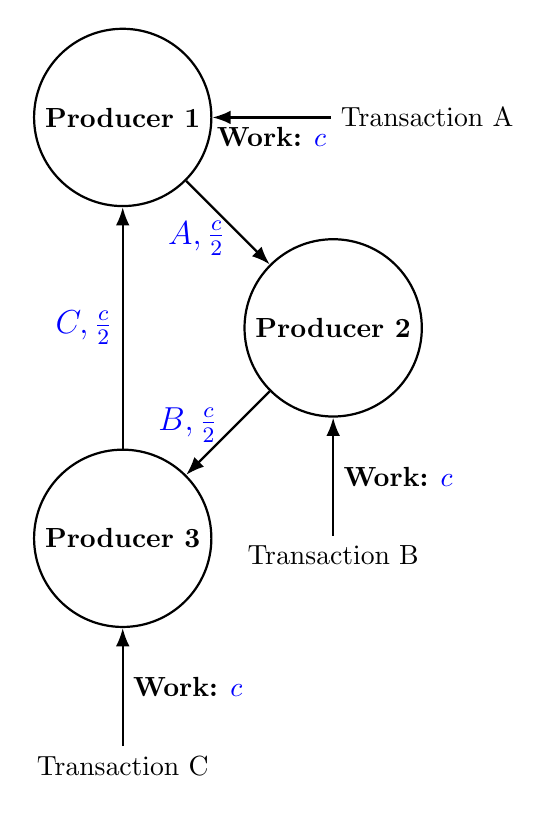
\begin{tikzpicture}[node distance=1.5cm, >=Latex, thick]

% block producers (BPs) positioned in a triangle
\node[draw, circle] (bp1) {\textbf{Producer 1}};
\node[draw, circle, below right=of bp1] (bp2) {\textbf{Producer 2}};
\node[draw, circle, below left=of bp2] (bp3) {\textbf{Producer 3}};

% Transactions
\node[right=1.5cm of bp1] (txA) {Transaction A};
\node[below=1.5cm of bp2] (txB) {Transaction B};
\node[below=1.5cm of bp3] (txC) {Transaction C};

% Routing Arrows (Transactions to Producers)
\draw[->] (txA) -- (bp1) node[midway, below] {\textbf{Work:} \textcolor{blue}{$c$}} ;
\draw[->] (txB) -- (bp2) node[midway, right] {\textbf{Work:} \textcolor{blue}{$c$}};
\draw[->] (txC) -- (bp3) node[midway, right] {\textbf{Work:} \textcolor{blue}{$c$}};

% Routing between Producers
\draw[->] (bp1) -- (bp2) node[midway, left, xshift=0.1cm,yshift=-0.2cm] {\large \textcolor{blue}{$A, \frac{c}{2}$}};
\draw[->] (bp2) -- (bp3) node[midway, left, yshift=0.1cm] {\large \textcolor{blue}{$B, \frac{c}{2}$}};
\draw[->] (bp3) -- (bp1) node[midway, left] {\large \textcolor{blue}{$C, \frac{c}{2}$}};

\end{tikzpicture}
    \caption{Illustrating Example~\ref{eg::ass1}}
    \label{fig::illustration}
\end{figure}


\paragraph{Change in $\alpha$ with Fake Transactions.}

In the above example, without fake transactions, the probability of winning for any block producer is $\alpha$. Assumption~\ref{assumption::1} states that for a sufficiently large set of outstanding transactions, such a scenario is mimicked. Thus, we follow Roughgarden in assuming that each honest block producer has the same winning probability. 

%
% we don't need each block producer to have the same probability of winning the next block as long as we can assume -- Roughgarden Compatibility -- that the allocation must happen without changing the probability of the block producer being selected.
%

With fake transactions, any block producer $i$ can only affect $S_i$, its own set of transactions. Thus, $\Pr(\mathbb{I}=1|S_i)$ will change. Formally, we can capture the change as $\Delta(\alpha) = \frac{\partial \alpha}{\partial \Pr(\mathbb{I}_i = 1| S_i)}$. From Eq. \ref{eqn:alphai}, we trivially observe that,

\begin{equation}\label{eqn:delta-alpha}
    \Delta(\alpha) = \frac{\partial \alpha_{i}}{\partial \Pr(\mathbb{I}_{i} = 1| S_{i})} = \Pr(S_{i})
\end{equation}

From Assumption \ref{assumption::1}, each block producer has the same probability of proposing the next block, so we have $\Pr(S_{i}) = \mathcal{O}\left(\frac{1}{m}\right)$, $\forall i \in [m]$, where $m$ are the total number of block producers. 

With this background, Lemma~\ref{lemma:fake-txn} shows that \ourTFM\ disincentivizes creation of fake transactions. 

\begin{lemma}
    In \ourTFM, as $m \to \infty$, including any fake transaction to compute $S$ (refer to \ourOPT) is disincentivized for any block producer $i \in \mathcal{P}$ if $\alpha \leq \frac{2}{k+1}$.
    % , the inclusion of $z$ fake transactions is disincentivized if 
    % $$ \alpha  \leq \frac{z - \epsilon/\tilde{p}}{|\tilde{S}| + z - |S| \frac{p}{\tilde{p}}} $$
    % \[
    % \alpha \leq \frac{z/k - \epsilon/(kp^{max})}{(1 - \frac{p}{\tilde{p}}) + z/k}
    % \]
    % and, 
    % \[
    % \frac{\partial \alpha}{\partial Pr(\mathbb{I}_{i} = 1 | S = S_{i}}) \leq \frac{2\epsilon}{\left(|\tilde{S}|\tilde{p} + c\tilde{p}\right)}
    % \]
    % hold true $\forall z \in [0,k]$, where $k$ is the block capacity. 
    % \sankarshan{not needed >>>>}
    % Here, $S$ is the set of transactions determined by the honest allocation rule, and $\tilde{S}$ is the set that includes $z$ fake transactions. 
    % $p^{max} = \max_{(t,h) \in S} t$ is maximum fees transaction, $p = \min_{(t,h) \in S} t$ is price setting transaction and $\epsilon$ diminishes by $\mathcal{O}\left(\frac{1}{m}\right)$ for $m$ block producers.  
    \label{lemma:fake-txn}
\end{lemma}
\begin{proof}
    Consider a block producer $i$ with $S \in$ \ourOPT, i.e., set of transactions selected for allocation. A strategic producer instead can choose an alternate subset $\tilde{S} \in \mathcal{M}_i \cup \mathcal{F}$ that includes a set of fake transactions, $\mathcal{F}$. Note that $\tilde{S}$ must also clear the routing work threshold and be within the block capacity. Let $p$ be the second-price payment per transaction when $S$ is published, and $\tilde{p}$ be the payment per transaction when $\tilde{S}$ is published. 
    
    % \varul{Since fake transactions included by block producer $i$ is incentivized only when they are selected out of $m$ potential block producer. We analyse utilities of honest and dishonest strategies in the case to show fake transaction inclusion is disincentivized.}

    Producer $i$'s utility without fake transaction is given by,
    $
    u_i = \alpha\cdot \frac{p}{2}\cdot |S|.
    $
    The utility corresponding to $\tilde{S}$ is given by,
    $$ \tilde{u}_i = (\alpha + \Delta \alpha) (|\tilde{S}| - z) \frac{\tilde{p}}{2}  -  (1-\alpha - \Delta \alpha) z \cdot \tilde{p} $$ where $\Delta \alpha$ is the change in the probability of winning the revenue lottery when $i$ unilaterally deviates and includes fake transactions.  The first term in $\tilde{u}$ corresponds to the payment $i$ receives when it wins the lottery with probability $(\alpha + \Delta\alpha)$. The second term corresponds to the payment lost when it loses the lottery. 
    
    The producer $i$ will not include fake transactions only when $\tilde{u}_i - u_i \leq 0$. That is,
 
    
    \begin{equation*}
    \begin{aligned}
        \tilde{u}_i - u_i & = |\tilde{S}|\cdot \frac{\tilde{p}}{2}(\alpha + \Delta \alpha) - (1 - \alpha - \Delta \alpha)\cdot z \cdot \tilde{p} \\ 
        & - (\alpha + \Delta \alpha)\frac{z\tilde{p}}{2} - |S|\frac{p}{2}\alpha\\
        & = \alpha \left(\frac{|\tilde{S}|\tilde{p}}{2} - \frac{|S|p}{2} + z\tilde{p} - \frac{z\tilde{p}}{2}\right) - z\tilde{p}  + \Delta \alpha \left(\frac{|\tilde{S}|\tilde{p}}{2} + \frac{z\tilde{p}}{2}\right) \\ 
        & \leq \alpha \left(\frac{|\tilde{S}|\tilde{p}}{2} - \frac{|S|p}{2} +\frac{z\tilde{p}}{2}\right) - z\tilde{p} + \epsilon 
    \end{aligned}
    \end{equation*}
    where $\epsilon \geq \Delta \alpha \left(\frac{|\tilde{S}|\tilde{p}}{2} + \frac{z\tilde{p}}{2}\right)$. To derive the condition for disincentivizing inclusion of fake transactions, i.e., $\tilde{u}_i - u_i \leq 0$, we have,
    
    % This is a reasonable assumption because $\Delta \alpha$ diminishes as number of block producers increase by $\mathcal{O}\left(\frac{1}{m}\right)$. The multiplicand $\left(\frac{|\tilde{S}|\tilde{p}}{2} + \frac{c\tilde{p}}{2}\right) $ is independent of $m$ and hence the term becomes smaller than $\epsilon$ for sufficiently large number of block producers. The condition therefore becomes 
    
    \begin{equation}\label{eqn:alpha}
    \alpha \leq \frac{z\tilde{p} - \epsilon}{\left( \frac{|\tilde{S}|\tilde{p}}{2} - \frac{|S|p}{2} + \frac{z\tilde{p}}{2}\right)} = \frac{2z\tilde{p} - \Delta\alpha \tilde{p} (|\tilde{S}| + z)}{\tilde{p} (|\tilde{S}| + z) - |S|p}
    \end{equation}

    As we saw before, $\Delta \alpha = \mathcal{O}(\frac{1}{m})$, with increasing number of block producers. Hence, $\epsilon$ diminishes with increase in number of block producers, $m$. We re-write Eq.~\ref{eqn:alpha} as,
    
    $$ \alpha  \leq \frac{2z - \Delta\alpha (|\tilde{S}| + z)}{|\tilde{S}| + z - |S| \frac{p}{\tilde{p}}} $$
    When $m \to \infty$ and $|\tilde{S}| \leq k$, $\Delta \alpha \to 0$. With trivial manipulations, 
    $$ \alpha \leq \frac{2z}{k + z}$$
    As the above inequality is increasing in $z\in\mathbb{N}$, if $\alpha \leq \frac{2}{k+1}$, the producer is not incentivized to include even a single fake transaction.  
    % \approx  \frac{z/k - \epsilon/(\tilde{p}k)}{(1 - p/\tilde{p}) + z/k}$$
    % where $k = |S| = |\tilde{S}|$ is the block capacity. 
   % $$ 
    \end{proof}
    \if 0
    However, selection of winner for transaction fees is done by (1) selecting one of $|\tilde{S}| + c$ transactions uniformly at random and then selecting one of the routers proportional to their routing work. Fake transactions are only routed by the block producer. Hence, probability of block producer being winner of payment lottery is $\geq \frac{c}{|\tilde{S}| + c}$. Therefore, $\frac{c}{|\tilde{S}| + c} \leq \alpha$, and for ensuring $U_{advr} - U_{honest} \leq 0$ we require Equation~\ref{eqn:alpha} to hold. This can be simultaneously satisfied only if $\forall c \exists \alpha$ such that 
    \begin{equation}\label{eqn:alpha-left-right}
        \frac{c}{|\tilde{S}| + c} \leq \alpha \leq \frac{c\tilde{p} - \epsilon}{\left( \frac{|\tilde{S}|\tilde{p}}{2} - \frac{|S|p}{2} + \frac{c\tilde{p}}{2}\right)}
    \end{equation}
    RHS is minimized when $\tilde{p} = p^{max}$. There exists such an $\alpha$ only if 
    \[
        \frac{c}{|\tilde{S}| + c} \leq \frac{c\tilde{p} - \epsilon}{\left( \frac{|\tilde{S}|\tilde{p}}{2} - \frac{|S|p}{2} + \frac{c\tilde{p}}{2}\right)} 
    \]
    \[
        \left(|\tilde{S}| + c\right)\tilde{p} - |S|p \leq 2\left(|\tilde{S}| + c\right)\tilde{p} - \frac{\epsilon(|\tilde{S}| + c)}{\tilde{p}}
    \]
    \[
        \epsilon \leq \frac{\left(|S|p + (|\tilde{S}| + c)\tilde{p}\right)\tilde{p}}{(|\tilde{S}| + c)} 
    \]
    Since $\Delta \alpha \left(\frac{|\tilde{S}|\tilde{p}}{2} + \frac{c\tilde{p}}{2}\right) \leq \epsilon$, we get
    \[
    \Delta \alpha \leq \frac{2\tilde{p}\left(|S|p + |\tilde{S}|\tilde{p} + c\tilde{p}\right)}{(|\tilde{S}| + c)^{2}}
    \]
    Since RHS is independent of $m$ (number of block producers), and LHS diminishes by $\mathcal{O}\left(\frac{1}{m}\right)$ with large enough number of producers, this condition is satisfied. This in-turn means there exists valid value of $\alpha, \forall c$ for which  Equation~\ref{eqn:alpha-left-right} is also satisfied. Such an $\alpha$ is set by the protocol through selection of $\tau$ (routing work threshold) protocol. 
    \fi


% %%%
\paragraph{Note.}
From Lemma~\ref{lemma:fake-txn}, we require $\alpha \leq  \frac{2}{k+1}$ when we burn $\frac{1}{2}$ of the payment (refer to Eq.~\ref{eqn::burn}). In general, for burning $f_b$ fraction of the total payments collected, we can re-write the bound by,
$$ \alpha \leq \frac{z}{k + (z-k)f_b}$$ From the above equation we can verify that, burning everything, i.e., $f_b = 1$ prevents inclusion of fake transactions universally, as expected. When $f_b = 0$, $\alpha$ increases slightly since the cost of a fake transaction reduces, formally, $\alpha \leq \frac{1}{k}$.
%%%%


\iffalse
\begin{lemma}\label{lemma:fake-txn}
    Inclusion of $z$ fake transaction $tx_{fake} = (f_{fake},h)$ for any $h$ is disincentivized for block producer if $\forall (f,h) \in S$
    \[
        Pr_{S} \leq \frac{\epsilon + (1 - \alpha)zf_{fake}}{(f_{fake} - f_{min})|S|}
    \]
    where, $Pr_{S}$ is the probability for the miner being selected as the winner of golden ticket reward for current block and $f_{min} = \min_{(f,h) \in S} f$ and $1 - \alpha$ of the transaction fees is burnt.
\end{lemma}
\begin{proof}
    Consider a block with transaction set $S$ included in the block. The block producer has replaced $z$ transactions with fake transactions to make the new set $S^{'}$. Note that $|S| \geq |S^{'}|$. \sankarshan{why should this hold? 2 fake txs can give the same routing work as 3 honest txs.}

 Consider blocks containing transaction sets $S$ and $S^{'}$ be $B$ and $B_{S^{'}}$ respectively. Consider $f_{min} = \min_{(f,h) \in S} f$ and $f_{fake} = \min_{(f,h) \in S^{'}} f$. Let the change in utility is $\Delta u = $ utility from producing block with $S^{'}$ $ - $ utility from producing block with $S$. Further, if the probability of block producer being winner of golden ticket for $B_{S}$ is $Pr_{S}$ and probability with $B_{S^{'}}$ is $Pr_{S^{'}} = Pr_{S} + \Delta p$. \sankarshan{This is non-intuitive. Golden ticket is just finding a random nonce. How is changing tx sets improving my probability of finding it?}


 Further, $F_{old} = \sum_{(f,h) \in S} f$ and $F_{new} = \sum_{(f,h) \in S^{'}} $ \sankarshan{$f$} are sum of transaction fees. \sankarshan{is $\Delta u$ for second-price payments?}
    \begin{equation*}
        \begin{aligned}
            \Delta u = &  \alpha Pr_{S^{'}}|S'|f_{fake} - \alpha Pr_{S}|S|f_{min} - z f_{fake}\\
            \leq &  \alpha Pr_{S^{'}}|S|f_{fake} - \alpha Pr_{S}|S|f_{min} - z f_{fake}\\
            = & \alpha Pr_{S}|S|\left(f_{fake} - f_{min}\right) + \alpha \Delta p|S|f_{fake} - z f_{fake}
        \end{aligned}
    \end{equation*}
\sankarshan{Ok, it seems by 'golden ticket' you actually meant the probability of being selected via the distributions created using fees and routing work. David uses golden ticket for the puzzle. Still the equation $Pr_{S^{'}} = Pr_{S} + \Delta p$ is not clear to me. Do we not have to do something like: $\mathbb{E}[\Delta u] = \mathbb{E}[\text{utility due to S} - \text{utility due to S'} ] = \mathbb{E}_{\sim S }[\text{utility due to S}] - \mathbb{E}_{\sim S'}[\text{utility due to S'}]$?   }

\sankarshan{So $\mathbb{E}_{\sim S }[u_S] = p_1 f_1 + \ldots + p_{|S|} f_{|S|}$ and $\mathbb{E}_{\sim S' }[u_{S'}] = p'_1 f'_1 + \ldots + p'_{|S'|} f'_{|S'|}$. But getting $\mathbb{E}[\Delta u]$ is hard as any 'swap' between txs changes probabilities of $p_1$ and $p'_1$ also. }

    The change in probability $\Delta p = \frac{z\cdot f_{fake}}{F_{new}} - \sum_{(f,h) \in S/S^{'}} \frac{f}{F_{old}}2^{-h}$. Therefore, 
        $$\Delta p \leq \frac{z\cdot f_{fake}}{F_{new}} - \frac{z \cdot f_{min}}{F_{old}} \leq \frac{z\cdot f_{fake}}{F_{new}}$$
        $$\Delta u = \alpha Pr_{S}|S|\left(f_{fake} - f_{min}\right) + \alpha\Delta p|S|f_{fake} - z f_{fake}$$
    The utility is at most marginally better if $\Delta u \leq \epsilon$. Using $\frac{f_{fake}|S|}{F_{new}} \leq 1$
    \begin{equation*}
    \begin{aligned}
        \Delta u \leq Pr_{S}|S|\left(f_{fake} - f_{min}\right) + \frac{\alpha z f_{fake}|S|f_{fake}}{F_{new}} - z f_{fake}\\
        \leq Pr_{S}|S|\left(f_{fake} - f_{min}\right) - (1 - \alpha)zf_{fake}\leq \epsilon  \\        
    \end{aligned}
    \end{equation*}
    Therefore, $Pr_{S} \leq \frac{\epsilon + (1 - \alpha)zf_{fake}}{|S|\left(f_{fake} - f_{min}\right)}$. 
    When the transaction pool is high enough, $\max_{(f,h) \in S} f - \min_{(f,h) \in S}f$ is very small. Therefore, $\frac{\epsilon}{(f_{fake} - f_{min})} \approx \mathcal{O}(1)$ and $\Delta u \leq \epsilon$ if $Pr_{S} \leq \frac{\epsilon + (1 - \alpha)zf_{fake}}{|S|\left(f_{fake} - f_{min}\right)}$.
        
\end{proof}
\fi 




















\textbf{Second,} in Lemma \ref{lemma:routing}, we show that \ourTFM\ also incentivizes block producers to propagate transactions. 
\textbf{Fourth,} Lemma~\ref{lemma:sybil-resistance} shows that block producers are not incentivized to create multiple identities to self-propagate transactions, i.e., to not launch a \emph{Sybil attack}. We combine Lemma~\ref{lemma:fake-txn} and Lemma~\ref{lemma:sybil-resistance} to show that \ourTFM\ is BPIC.

%
%%
%%%%%
\begin{figure}[t]
\centering
    \fbox{
     \centering \parbox{0.9\linewidth}{  % Box width
        \begin{enumerate}[leftmargin=*,itemsep=0.2em]
        \item \textbf{Allocation:} 
        A block producer $i\in\mathcal{P}$, with its local mempool $\mathcal{M}_i$,  confirms a set $S\subseteq \mathcal{M}_i$ by solving for \ourOPT. The optimization \ourOPT\ constraints $S$ to clear the routing threshold $\tau$ and honor the block capacity $C$. 
    
        \item \textbf{User Payment Rule:} Each confirmed user, $b_j \in S$, pays the minimum confirmed bid, i.e., $p_j = \min_{(b_t,h_t)\in S} b_t$. The remaining users $\mathcal{M}_i\setminus S$ pay zero.
    
        \item \textbf{Block Burning Rule:} From the total user payments, $\sum_{(b_t,h_t)\in S} p_t$, we burn $\frac{1}{2}$ fraction of it. That is, the total payment burned is $\delta(S) = \frac{1}{2} \sum_{(b_t,h_t)\in S} p_t$.
    
        \item \textbf{Block Producer Revenue Rule:} Once a block is produced, an \textit{on-chain lottery} determines the routing node that receives the remaining collected payment (post-burning), $\frac{1}{2} \sum_{(b_t,h_t)\in S} p_t$. 
        
        To select the node that receives the payments, the lottery (i) uniformly samples a transaction from $S$ and (ii) uniformly selects a hop from the routing path of the sampled transaction. The node corresponding to the selected hop receives $\frac{1}{2} \sum_{(b_t,h_t)\in S} p_t$. 
        
        % The payment is not always made to the block producer, but the block producer may be selected as the winner in the lottery.
        % The chance of each transaction winning is weighted according to its share of all fees in the block. That hash is then hashed again to select a hop from the routing path of the winning transaction, with each hop weighted according to its share of work in the overall routing path.
        \end{enumerate}
      }
    }
    \caption{\ourTFM: Mechanism Outline}\label{fig::rtr-tfm}
\end{figure}
%%%%%
%%%
%%






\subsection{\ourTFM: Allocation, Payments and Burning Rules\label{subsec::block-production}}

\noindent \textbf{Transactions.} Recall from Section~\ref{sec::prelims}, that each transaction received by the block producer $i\in \mathcal{P}$ is denoted by the tuple $(b,h) \in \mathcal{M}_i$. That is, the bid $b \in \mathbb{R}_{\geq 0}$ submitted by a user, and the corresponding routing hops $h \in \mathbb{N}$ each transaction has gone through before reaching the producer $i$. We also assume that each transaction has the same size, as a shortcut to normalize fees-per-byte and avoid the need to adjust the likelihood of any transaction winning the payout lottery to its relative contribution of fees to the block.

\noindent \textbf{Routing Work.} We now define the routing work for any transaction $(b,h) \in \mathcal{M}_i$. Consider a function $\omega:\mathbb{R}_{\geq 0}\times\mathbb{N}\rightarrow\mathbb{R}_{\geq 0}$ that represents the amount of routing work gained by a block producer at the $h\textsuperscript{th}$ hop. In \ourTFM, the routing function $\omega$ is:
\begin{equation}
    \omega(h) := c\cdot2^{1 - h}
\end{equation}
That is, \ourTFM\ offers 1\textsuperscript{st}-hop nodes $c\in \mathbb{R}_{\geq 0}$ units of routing work, 2\textsuperscript{nd}-hop nodes $\frac{c}{2}$ units of routing work, 3\textsuperscript{rd}-hop nodes $\frac{c}{4}$ units of routing work, and so on.

\noindent \textbf{Allocation Rule.} Each producer $i\in \mathcal{P}$ selects transactions from $M_i$ by solving the following optimization, denoted by \ourOPT,
\begin{align}\tag{\ourOPT}
    \begin{rcases}
        \underset{S\subseteq \mathcal{M}_i}{\mbox{arg}\max} & \min_{(b_t,h_t)\in S}  b_t \\
       \mbox{{s.t.}}\  & \sum_{(b_t,h_t)\in S} \omega(h_t) \geq \tau \\
       & |S| \leq k\\
   \end{rcases}
\end{align}

The first constraint ensures that $S\subseteq \mathcal{M}_i$ clears the \textit{network-determined threshold for routing work}, $\tau$\footnote{The threshold $\tau$ is a network-determined dynamic parameter and increases upon block production, and slowly decreases until the next block is produced, similar in principle to the role of the base fee in EIP-1559~\cite{buterin2019eip}. As we consider myopic block producers and users, we omit additional details on the role of $\tau$.}. For the second constraint, recall that each transaction is of the same size. This implies that the total transactions in a block cannot exceed its capacity, $|S| \leq k$. Throughout this paper, we refer to $S\subseteq \mathcal{M}_i$ as the subset that satisfies these two constraints and $S^\star$ as the solution to \ourOPT.

\paragraph{User Payment Rule.} As aforementioned, while the second-price auction is incentive-compatible for users, in TFMs, the block producers are also strategic. Producers can inflate the highest-losing (price-setting) bid to maximize their revenue. To avoid such strategic manipulations by the producers, and as payments can only depend on the transactions part of the block, in \ourTFM, we let confirmed transactions pay a fee equal to the lowest confirmed bid. That is, $\forall (b_t,h_t)\in S$, we have 
\begin{equation}
    p_t := \min_{(b_t,h_t) \in S} b_t
\end{equation}

For the confirmed transaction with the lowest bid, the auction becomes a first-price auction, thus compromising IC on the user end. \citet{roughgarden2021} argues that such a payment rule is approximately-UIC, given a sufficiently large transaction pool.

\paragraph{Burning Rule.} In TFMs, a certain fraction of a cryptocurrency's supply is often burned, i.e., removed from circulation. This can be done by having the consensus mechanism issuing less in payouts than have been collected in network fees. While it is theoretically possible to improve on this lower bound, we set the fraction of network fees that are burned in \ourTFM as $1/2$ for purposes of this paper, i.e., 
\begin{equation}\label{eqn::burn}
    \delta(S) := \frac{1}{2} \sum_{(b_t,h_t)\in S} p_t
\end{equation}

\subsection{\ourTFM: Producer Revenue rule\label{subsec::producer-revenue}}
While half of the transaction fees are burned in \ourTFM, the other half is paid to a random node from set of nodes identifiable from the routing paths within the set of transactions included in the block. This is in contrast to existing (popular) TFMs that give the surplus directly to the block producer.

\noindent \textbf{Block Producer Revenue Rule. } A block can be produced only when it has enough transactions to meet the routing threshold, $\tau$. From \ourOPT, a producer $i \in \mathcal{P}$ computes $S \subseteq \mathcal{M}_i$, such that the transactions in $S$ clear $\tau$, or, 
$$
\sum_{(b_t,h_t) \in S} \frac{c}{2^{j-1}} \geq \tau.
$$

In \ourTFM, we employ the second-price payment rule. That is, the payment collected from \emph{each} user whose transactions are confirmed in $S$ is the lowest winning bid (say) $p$. The total payment collected is $\frac{1}{2}\cdot|S|\cdot p$ (recall that the other half is burned). However, the block producer is not guaranteed to receive the payment when the block is produced. Instead, the payment is made through a \textit{revenue lottery}, defined formally in Figure~\ref{fig::payment}.

\begin{figure}[h]
\centering
    \fbox{
     \centering \parbox{0.9\linewidth}{  % Box width
     The revenue, $\frac{1}{2}\cdot|S|\cdot p$, collected when a block is produced is given to the winner sampled from the following distribution. All sampling is done on-chain, i.e., in a trusted manner~\cite{chung2023foundations,damle2024designing}.
        \begin{enumerate}[leftmargin=*,itemsep=0.2em]
            \item Sample a transaction $t^\star \in S$ uniformly, i.e., $t^\star \sim \text{Uniform}(S)$.
            \item From the routing path of $t^\star$, sample a node through a probability distribution that weighs each node by their share of the routing work available at their hop over the total sum of routing work available to all nodes in the routing path of the transaction as included in the block.
                \begin{itemize}
                    \item Let the producers part of $t^\star$'s routing path be (w.l.o.g.) $\mathbf{P}_{t^\star}=\{1,\ldots,l\}$.
                    \item Any producer's $i \in \mathcal{P}_{t^\star}$ routing work for the transaction $t^\star$ is $\omega(t^\star;h_{i})$. Likewise, the total routing work for $t^\star$ is $\sum_{i \in \mathcal{P}_{t^\star}} \omega(t_\star;h_{i})$.
                    \item We sample a producer $i^\star \in \mathcal{P}_{t^\star}$ from the following weighted probability distribution:
                        $$
                        \Pr(i^\star) \sim \frac{\omega(t^\star;h_{i^\star})}{\sum_{i \in \mathcal{P}_{t^\star}} \omega(t_\star;h_{i})}
                        $$
                    \item The producer $i^\star$ receives the payment $\frac{1}{2}\cdot|S|\cdot p$.
                \end{itemize}
        \end{enumerate}
      }
    }
    \caption{\ourTFM: Revenue Lottery given $S$ (refer \ourOPT)}\label{fig::payment}
\end{figure}

We provide a working example of the revenue lottery in Figure~\ref{fig::teaser}. For instance, from Figure~\ref{fig::teaser}, if a transaction is sampled that was proposed by the second node to receive it, then this transaction has two nodes in its routing path. The total routing work for all nodes in the routing path is $c+\frac{c}{2}=\frac{3c}{2}$. The sampling probability of the first-hop node is $\frac{c}{3c/2}=\frac{2}{3}$ while the sampling probability of the second-hop node is $\frac{c/2}{3c/2}=\frac{1}{3}$. 

\iffalse

\noindent \textbf{Routing Threshold and $\alpha$}













\paragraph{Winning the Revenue Lottery.}
In \ourTFM, the block producers are simultaneously working towards block production, i.e., solving \ourOPT. Let $S_i$ be the output of \ourOPT\ for a producer $i\in\mathcal{P}$. If the block producer $i$ is successful, $S_i$ gets confirmed. The revenue of the block is given to a producer using the revenue lottery (Figure~\ref{fig::payment}). Note that any block producer may have a chance to receive the revenue as long as it is in the routing path of one of the confirmed transactions. The probability of an arbitrary producer $i$ receiving the revenue, denoted by $\alpha_i$ may be written as,

\begin{equation}\label{eqn:alphai}
    \alpha_{i} = \sum_{j = 1}^{m} \Pr(\mathbb{I}_{i} = 1 | S_{j})\cdot \Pr(S_{j})
\end{equation}

Here, the indicator variable  $\mathbb{I}_{i} = 1$ denotes the event that producer $i$ is selected as the winner (recipient) of the block's payment; $\mathbb{I}_{i} = 0$ otherwise. $\Pr(S_j)$ denotes the confirmation of the set $S_j$ owned by the $j^{\mbox{th}}$ producer. 


\if 0
\begin{itemizerally dev\tilde{iates from proposing $S_$e}
    \{i}item If this transaction is confirmed in the block, then auction becomes a first price auction for this transaction (compromising IC on the user end). 
    \item If this transaction is included but not confirmed in the block, the miner is incentivized to include \emph{fake transaction} in the block to increase the price setter transaction to strategically increase its revenue. 
\end{itemize}
We therefore come up with a proposal to use \emph{verifiable on-chain randomness} to \st{include} \sankarshan{confirm} the \sankarshan{price-setting} transaction in the block with certain probability which is $p_{conf}$. 
% in decreasing order of $f\cdot\omega(f,h)$ values. 

\noindent \textbf{Second Price Payment Rule.} All \st{included} \sankarshan{confirmed} transactions pay the \st{least accepted transaction fee} \sankarshan{lowest confirmed bid??}. The \emph{price setter} transaction is \st{included} \sankarshan{confirmed} with probability $p_{conf}$ and is part of payment to the \st{miner} \sankarshan{block producer}. Otherwise, it is not part of the payment to \st{block} \sankarshan{the} producer. Consider $\mathbb{I}_{incl} = 1$ if price setter is \st{included} \sankarshan{confirmed} and $0$ otherwise. The total payment from the block is 
\begin{equation}\label{eqn:payment-total}
    F = (|S\sankarshan{|} - 1 + \mathbb{I}_{incl}) \min_{(f,h) \in S} f
\end{equation}

The payment is divided into two parts: $p = (p_{solver}, p_{winner})$ where (1) $p_{solver}$ goes to the player who solves \emph{golden ticket} (if there are no solvers, this payment is burnt) and (2) $p_{winner}$ goes to a randomly chosen router out of the set of transactions included in a block according to the \emph{golden ticket winner selection} (described in the the following section). Out of the total transaction fees in a block, $\alpha$ $\in [0,1]$ fraction goes to $p_{winner}$ and $(1 - \alpha)$ to $p_{solver}$. 
\begin{equation}\label{eqn:payment-winner}
p_{winner} = \alpha\cdot(|S - 1| + \mathbb{I}_{incl}) \cdot  \min_{(f,h) \in S} f  
\end{equation}


\noindent \textbf{Golden Ticket.} Golden ticket for a block is solved by a player (say) $solver$ in the next block and gets $(1 - \alpha)F$ and the result of the golden ticket. Consider the probability with which the golden ticket is solved in the next block be $\phi$. Payment to the solver is

\[
    p_{solver} = 
\begin{cases}
(1 - \alpha)F \hspace{20pt} \text{with probability $\phi$}\\
0 \hspace{45pt} \text{otherwise}
\end{cases}

\]

\noindent \textbf{Golden Ticket Winner Selection.} The solution of golden ticket is a random variable that decides another player (router from the current block) $winner$ (say) who gets remaining $\alpha$ fraction of the transaction fee from the block (See Equation~\ref{eqn:payment-winner}). $p_{winner}$ is paid $\alpha$ fraction of  to one of the routers from all transactions contained in the block. The probability of any transaction $tx = (f,h) \in \mathcal{B}$ getting selected is $\frac{f}{F}$ and the probability of router $j \in [1,h]$ getting selected is $\frac{2^{-j}}{(1 - 2^{-h})}$.

\noindent \textbf{Burn Rule $q$.} The burn rule is to burn the payment designated for $solver$ of golden ticket if the puzzle for a block is not solved in the immediate block. Such a case happens with probability $1 - \phi$. The burn rule is therefore, 

\[
q = \begin{cases}
        (1 - \alpha)F \hspace{20pt} \text{with probability $1 - \phi$}\\
        0 \hspace{20pt} \text{otherwise}
    \end{cases}
\]

The transaction fees mechanism is therefore represented as $\mathcal{T}_{route} = \langle x_{incl}, (p_{solver},p_{winner}), q \rangle$.
\subsection{Utility}
\subsubsection{User Utility} User proposes a transaction $tx$ and has some valuation that they get when this transaction gets accepted in the current block. Consider user with transaction $tx$ with valuation $\overline{f}$ and disclosed bid (in form of transaction fees) as $f$. The set of transactions accepted in the current block is contained in set $S$, then the utility for user is represented as
\begin{equation}
    u(tx,\overline{f}) = \begin{cases}
        f - \overline{f} \hspace{20pt}\text{if }tx \in S\\
        0 \hspace{35pt}\text{otherwise}
    \end{cases}
\end{equation}
\subsubsection{block producer Utility} 
\subsection{Incentive Compatibility}
\begin{definition}[User Incentive Compatibility (UIC)]\label{def:UIC}
    
\end{definition}


\begin{definition}[Miner Incentive Compatibility (MIC)]\label{def:MIC}
    
\end{definition}

\fi


Having presented the formal protocol in Section~\ref{sec::protocol}, in this section, we now game-theoretically prove \ourTFM achieves Roughgarden Compatibility for both users and block producers.





 





\subsection{\ourTFM: Traditional Incentive Compatibility}

In addition achieving Roughgarden Compatibility, \ourTFM also achieves traditional incentive compatibility. In order to demonstrate this, we define our \textit{social choice rule}, and then demonstrate the profit-maximizing behavior of all rational actors leads to this socially-optimal outcome.

We choose \textit{pareto optimality} as our \textit{social choice rule}. This refers to the point of production defined by the equation below, where we cannot increase utility for any individual without decreasing it for at least one other participant. This by definition puts overall production on the \textit{production possibilities frontier}, which means that the blockchain is being produced and funded at optimal levels relative to the utility it provides participants relative to all other goods and services competing for consumption of the same fee.

\textit{Pareto optimality} is the appropriate social choice rule not only because it means the blockchain is producing utility with the highest possible efficiency, but because it eliminates the . Given that all participants are voluntarily optimizing their resource-allocation strategies at this point, \textit{pareto optimality} makes all forms of user-user and producer-producer collusion impossible: no subset of participants can change their individual decisions regarding resource allocation without shifting to a less desirable equilibrium.

Setting \textit{pareto optimality} as our \textit{social choice rule} thus aligns social optimality with maximum utility for user, and reduces the scope of potentially profitable collusion to the case of user-producer collusion.

We observe that \ourTFM achieves traditional incentive compatibility. This can be done extremely simply, merely by observing the nature of competition and price-discovery in the network and seeing that it aligns with the 

\subsection{\ourTFM: Traditional Incentive Compatibility}

We can prove incentive compatibility easily by observing that \ourTFM falls into the category of two-sided competitive markets.



Competitive markets with multiple consumers and multiple producers are known to be incentive compatible








\paragraph{Sybil-attacks are Disincentivized.} We discuss the block producer's incentive for launching Sybil-attack in Lemma~\ref{lemma:sybil-resistance}.

\begin{lemma}\label{lemma:sybil-resistance}
   Under Assumption~\ref{assumption::1}, not launching a Sybil attack is a Nash equilibrium strategy for block producers in \ourTFM.
\end{lemma}
\begin{proof}
    Consider any block producer $i\in\mathcal{P}$ and a transaction $tx = (b,h)$ that reaches $i$ after $h-1$ hops. Now, the producer has two strategies: (1) to launch a Sybil-attack and (2) not to launch one. Recall that to launch a Sybil attack, the producer propagates transactions to itself, by creating multiple identities. For the proof, we show launching a Sybil attack is not a Nash equilibrium strategy if a block producer $i$ propagates a transaction to multiple identities it owns and \underline{Case 1} --- broadcasts the propagated transaction and \underline{Case 2} --- includes this transaction in their block.
    
    \smallskip\noindent\textbf{\underline{Case 1:}} If this transaction is broadcasted and later added to the proposed block by another block producer $j$, there might be an increased probability of Producer $i$ winning the revenue lottery due to existence of its own pseudo identities in the routing path. Let this increase be $x$ to the utility. If the transaction gave utility $u$ to $i$ (in expectation) if the non-Sybil transaction is included by block producer $j$, then utility (in expectation) is $u + x$ for Sybil transaction. 

    If all other block producers follow non-Sybil strategy, there exists with high probability another (non-Sybil) router through which $j$ gets the same transaction with lesser hops. They are incentivized to include this transaction instead of transaction broadcasted by $i$.
\begin{table}[]
\begin{center}
\begin{tabular}{ | m{4em} | m{5em}| m{4em} | } 
    \hline
         & \textbf{Sybil} & \textbf{Not Sybil} \\ 
        \hline
        \textbf{Sybil} & $(u+x,u+x)$ & $(0,u)$ \\ 
    \hline
        \textbf{Not Sybil} & $(u,0)$ & $(u,u)$ \\ 
    \hline
\end{tabular}
\end{center}
    \caption{Game between Sybil and Non-Sybil Strategy}
    \label{tab:induced-game}
\end{table}
    The game induced is summarized in Table~\ref{tab:induced-game}. We see that the "Not-Sybil" strategy is Nash Equilibrium for the Producer.  

    \smallskip\noindent\textbf{\underline{Case 2:}} In this case, if there are $|S|$ total transactions in the block produced by $i$, then by adding multiple identities with a Sybil attack, the total routing work reduces. E.g., signing on transaction $tx = (b, h)$ a total of $z$ times reduces total work contributed by this transaction by a factor of $\frac{1}{2^{z}}$. To compensate for this reduced work, fake transactions must be added by the producer such that the total routing work satisfies the threshold. This fake transaction is therefore $tx_{fake} = (b_{min},1)$ where $b_{min} = \min_{(b, h) \in S} b$. Out of this, $\frac{b_{min}}{2}$ is burnt, which is the negative payment. Improvement in utility due to sybil attack is therefore, $\Delta u = |S|b_{min}\frac{\partial\alpha}{\partial \Pr(\mathbb{I}_{i} = 1 | S)} - \frac{b_{min}}{2}$. Note that $\frac{\partial\alpha }{\partial \Pr(\mathbb{I}_{i} = 1 | S)} = \Pr(S)$ diminishes by $\mathcal{O}\left(\frac{1}{m}\right)$. For sufficiently large number of block producers, $\Delta u < 0$, when $\Pr(S) < \frac{1}{2|S|}$. Hence for large number of block producers, sybil attack is disincentivized. 
\end{proof}


We now combine these results to show that \ourTFM\ is BPIC. 
% Consider the following theorem.

\begin{theorem}\label{thm::bpic}
    \ourTFM\ is block producer Incentive Compatible (BPIC) under Assumption~\ref{assumption::1}. 
\end{theorem}
\begin{proof}
    From the definition of BPIC (Definition~\ref{def::BPIC}), as the block producers are not incentivized (i) to include fake transactions (Lemma~\ref{lemma:fake-txn}) and (ii) to not launch a Sybil-attack (Lemma~\ref{lemma:sybil-resistance}). As the allocation rule is utility maximizing (\ourOPT), \ourTFM\ is BPIC.
\end{proof}


Table~\ref{tab::summary} tabulates the results presented in this section. In summary, we present a novel TFM that avoids free-riding and satisfies UIC and BPIC, under reasonable assumptions, and without any modifications to the utility structure.

\begin{table}[h]
    \centering
    \begin{tabular}{cc}
    \toprule
    \textbf{Property} &  \ourTFM  \\
    \midrule
    UIC     &  \cmark$^\dagger$~(Theorem~\ref{thm:UIC}) \\
    Transaction Propagation &  \cmark~(Lemma~\ref{lemma:routing})  \\
    Sybil-resistance   &  \cmark$^\ddagger$~(Lemma~\ref{lemma:sybil-resistance})    \\
    BPIC    &  \cmark$^\ddagger$~(Theorem~\ref{thm::bpic})  \\ 
    \bottomrule
    \multicolumn{2}{l}{$^\dagger$: Almost-UIC~\cite[Footnote 28]{roughgarden2021}} \\
    \multicolumn{2}{l}{$^\ddagger$: Under Assumption~\ref{assumption::1}}
    \end{tabular}
    \caption{\ourTFM: Results Summary}
    \label{tab::summary}
\end{table}





\emph{Transaction Fee Mechanisms} (TFMs) refer to a class of distributed systems in which a consensus mechanism governs the allocation of the same resource that it uses to incentivize its own provision. Unlike traditional mechanisms, where the number of honest and dishonest processes is static, in TFMs voting power is dynamic — it adjusts with the payouts issued by the mechanism. This introduces the ability for attacks intended to extract profits from this circular flow of funds to compromise the stability of the mechanism.

As more and more of these attacks have been identified in practice, computer scientists have typically named them after the "mechanism-specific" techniques they exploit, resulting in a wide array of terminology such as sybil attacks, block-orphaning attacks, selfish mining attacks, fee manipulation attacks, eclipse attacks, side-contract payments, and others. While most researchers treat these vulnerabilities as isolated technical challenges, a few scholars have applied concepts from mechanism design and economics to ask whether general solutions are possible. Unfortunately, this has led to a series of impossibility results that suggest socially optimal TFMs may be infeasible.

This paper challenges these results by identifying the exact equilibrium in which all such attacks are irrational. It argues that three distinct types of goal conflict -— self-interest, free-riding, and strategic manipulation —- are what prevent this equilibrium from being implemented by most \textit{TFMs}. We then review the earlier work in the field to show why they believe the problem is insolvable: their conclusions result from a reliance on auction models which limits their ability to address all three types of goal conflict or even handle the informational complexity necessary to compute the required equilibria.

Using the language of mechanism design, this paper demonstrates that the social choice rule needed to achieve fee-optimality and collusion-resilience is \textit{pareto optimality}, but the direct mechanisms used to model TFMs are incapable of implementing this rule, as doing so requires multi-dimensional preference revelation across a high-dimensional preference space -- a level of informational complexity that composable algorithms cannot handle. While Maskin's Revelation Principle teaches that a direct mechanism must exist for any indirect mechanism, in this case achieving optimality requires decomposable algorithms that use the "no-trade option" to reduce the complexity of computation and limit the scope of the state transitions proposed to those consistent with an efficiency shift towards \textit{paretop optimality}.

Since familiarity with economics is needed to understand what our three types of goal conflict are and why they exist, the next section of this paper begins by identifying the novel characteristics of TFMs, and showing how they create problems with self-interest, free-riding and strategic manipulation. We then show why \textit{pareto optimality} is the social choice rule needed to eliminate all three, which leads to a review of the impossibility results mentioned above and a discussion of how the conclusions of these papers reflect the informational limitations of the auction models they use to analyse the problem.

In the second half of this paper, we introduce a novel class of indirect mechanism that is theoretically compatible with \textit{pareto optimality}. We provide the formula for this mechanism and then a game-theoretic treatment of it which proves its inconsistency with the impossibility results discussed earlier, and demonstrates its ability to achieve otherwise intractable outcomes. We then close with a return to economic theory and discussion of how the mechanism overcomes the more foundational theoretical problems identified by Samuelson and Hurwicz to the attainment of incentive compatibility as a general economic problem.





% \newpage
% \section{Related Work\label{sec::rw}}
% \input{AAMAS25/sections/rw}

% \newpage
% \section{Preliminaries\label{sec::prelims}}
% \input{AAMAS25/sections/preliminaries}

% \newpage
% \section{\ourTFM: Routing-based Randomized TFM\label{sec::protocol}}
% \input{AAMAS25/sections/rtrtfm}

% \section{\ourTFM: Game-theoretic Characterization\label{sec::analysis}}
% \input{AAMAS25/sections/analysis}



% \newpage
\section{Conclusion \& Future Work}
In this paper, we introduced \textsc{RTR-TFM}: a novel TFM that addresses the incentive misalignment in classic transaction fee mechanisms (TFMs) by introducing a novel routing-based block production rule and a revenue scheme. \ourTFM\ rewards block producers in proportion to their contribution to the propagation of transactions. Such a reward ensures that block producers actively participate in the blockchain network upkeep instead of free-riding on other participating nodes. We also provide a game-theoretic characterization of the underlying game in \ourTFM. We prove that \textsc{RTR-TFM} effectively discourages transaction hoarding, ensures Sybil resistance, and achieves incentive compatibility for both users and block producers under reasonable assumptions.

\paragraph{Future Work.} With \ourTFM, we introduce a TFM revenue rule that links a direct cost to the block producers to create fake transactions. However, our BPIC analysis assumes a bootstrapped blockchain (Assumption~\ref{assumption::1}). While Assumption~\ref{assumption::1} is practical, we can look towards BPIC guarantees without constraints on the blockchain state. Furthermore, the TFM literature also looks at off-chain collusion between users and producers. \cite{gafni2024barriers} show the impossibility of a deterministic TFM simultaneously satisfying the UIC, the BPIC, and the resistance to off-chain collusion between a user and a producer. Future work can also study off-chain collusion guarantees for \ourTFM. 


% TO ADD: It is always incentivized to include block 
% Swap a transaction with a fake transaction 
% \url{https://docs.google.com/spreadsheets/d/1XVnXETZuQC0HijhT5H-Qh3CsxEc7fzhgJ_H2Xyq0GUM/edit?usp=sharing}


%%%%%%%%%%%%%%%%%%%%%%%%%%%%%%%%%%%%%%%%%%%%%%%%%%%%%%%%%%%%%%%%%%%%%%%%

%%% The next two lines define, first, the bibliography style to be 
%%% applied, and, second, the bibliography file to be used.
\cleardoublepage
\bibliographystyle{ACM-Reference-Format} 
\bibliography{ref}

%%%%%%%%%%%%%%%%%%%%%%%%%%%%%%%%%%%%%%%%%%%%%%%%%%%%%%%%%%%%%%%%%%%%%%%%

\end{document}

%%%%%%%%%%%%%%%%%%%%%%%%%%%%%%%%%%%%%%%%%%%%%%%%%%%%%%%%%%%%%%%%%%%%%%%%


